\chapter{Resultados}
\label{capitulo6}
\lhead{Capítulo 6. \emph{Resultados}}

En el capítulo anterior, se detalló la implementación de la solución propuesta para abordar el problema de evasión de obstáculos en QUAVs, centrándose en la metodología, la plataforma de implementación, la justificación del algoritmo seleccionado y la descripción del funcionamiento de los componentes principales. Este capítulo se adentra ahora en la evaluación y presentación de los resultados obtenidos, proporcionando una perspectiva crítica sobre el rendimiento de la solución propuesta.

En la Sección  \ref{sec:results-finetune} se examinan los resultados del ajuste fino de la política estudiante, destacando los desafíos asociados al sobre-ajuste de los datos de entrenamiento y a la generación de la base de datos. Además, se exploran las consecuencias derivadas de estos problemas al evaluar la política de evasión de obstáculos.

La Sección  \ref{sec:results-flights} examina los resultados de la política de evasión de obstáculos, dividida en dos subsecciones clave: la Sección  \ref{sec:results-AirSim}, que presenta los resultados de vuelos en simulación, y la Sección  \ref{sec:results-SOTEN}, centrada en vuelos sobre la plataforma física de implementación, SOTEN. Estos resultados ofrecen una perspectiva del rendimiento de la solución en configuraciones simples de obstáculos, cuya política de evasión se muestra estable. Además, se evalúan otras configuraciones de obstáculos en donde la política no logra completar su función de manera satisfactoria, y se identifica la relación entre este resultado y los desafíos asociados al ajuste fino de la política estudiante.

El análisis detallado de estos resultados proporciona una evaluación crítica de la efectividad de la solución propuesta, sirviendo como base para la discusión en el siguiente capítulo. Aquí, se extraerán conclusiones significativas y se identificarán posibles direcciones para mejorar el rendimiento en futuras investigaciones en el campo de evasión de obstáculos en QUAVs.

\section{Resultados del ajuste fino de la política estudiante}

\label{sec:results-finetune}

Como se mencionó en el capítulo anterior, el objetivo del ajuste fino de la política estudiante, es ajustar los pesos provistos por los autores del trabajo original \cite{Loquercio2021} para que la red neuronal genere trayectorias con \jim{v_{des} = 1} m/s; idealmente, manteniendo un nivel de generalización comparable a la red publicada en \cite{Loquercio2021}. Recordando que la función de pérdida de la red neuronal de la política estudiante tiene dos componentes: un componente espacial que cuantifica qué tan cerca se encuentran las trayectorias predichas a las generadas por el experto, y un componente de estimación que cuantifica que tan correctamente se hace la estimación del costo de ejecución \jim{c_k} \cite{Loquercio2021}; la Figura \ref{fig:loss-space-all} y la Figura \ref{fig:loss-estim-all} muestran el valor del componente espacial y de estimación en función de las épocas, tanto para el conjunto de entrenamiento como para el de validación.

\begin{figure}[H]
    \centering
    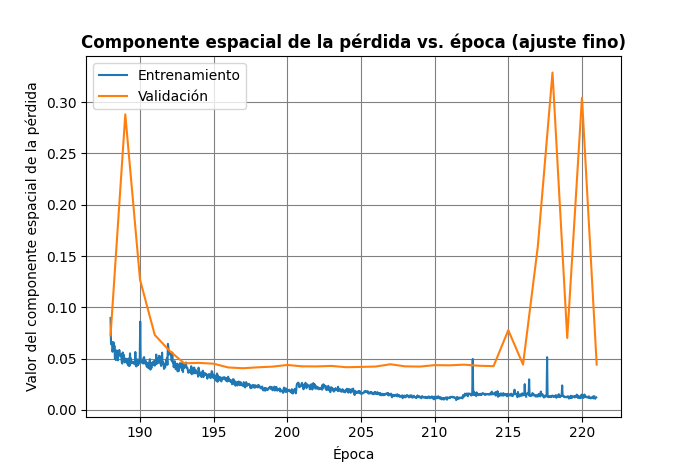
\includegraphics[scale=0.6]{partes/img/loss-space-all.png}
    \caption[Componente espacial de la pérdida vs. época (ajuste fino).]{Componente espacial de la pérdida vs. época (ajuste fino). Se observa claramente la divergencia de la pérdida sobre el conjunto de validación a partir de la época 215.}
    \label{fig:loss-space-all}
\end{figure}

\begin{figure}[H]
    \centering
    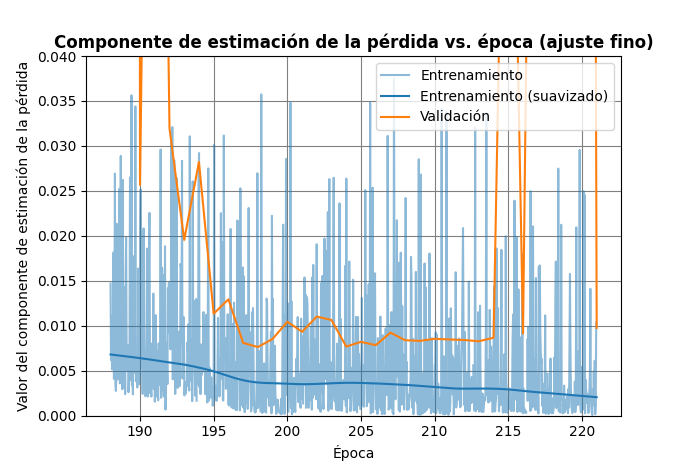
\includegraphics[scale=0.6]{partes/img/loss-estim-all.png}
    \caption[Componente de estimación de la pérdida vs. época (ajuste fino).]{Componente de estimación de la pérdida vs. época (ajuste fino). Se observa claramente la divergencia de la pérdida sobre el conjunto de validación a partir de la época 215.}
    \label{fig:loss-estim-all}
\end{figure}

La Figura \ref{fig:loss-space-all} y la Figura \ref{fig:loss-estim-all} reflejan la divergencia del valor de la pérdida sobre el conjunto de validación a partir de la época 215. Para contrarrestar este efecto, se decidió utilizar un punto de control temprano antes de la divergencia, efectivamente deteniendo el entrenamiento de forma temprana. El punto de control más cercano anterior a la época 215 fue el punto de control de la época 213. Al regresar a dicho punto de control se eliminó la divergencia del valor de pérdida de validación. La Figura \ref{fig:loss-space-stopped} y la Figura \ref{fig:loss-estim-stopped} muestran el valor del componente espacial y de estimación en función de las épocas luego de detener tempranamente el entrenamiento, tanto para el conjunto de entrenamiento como para el de validación. 

\begin{figure}[H]
    \centering
    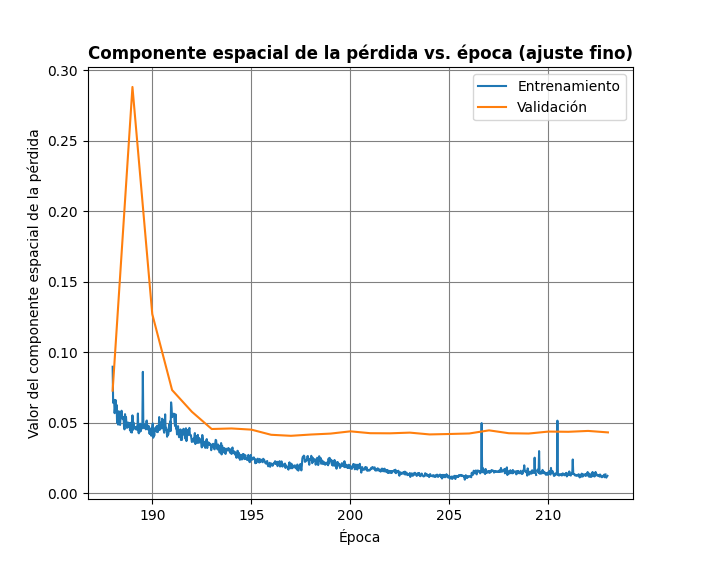
\includegraphics[scale=0.6]{partes/img/loss-space-stopped.png}
    \caption[Componente espacial de la pérdida vs. época (ajuste fino) luego de detener el entrenamiento tempranamente.]{Componente espacial de la pérdida vs. época (ajuste fino) luego de detener el entrenamiento tempranamente. No se observa divergencia en el valor de la pérdida sobre el conjunto de validación.}
    \label{fig:loss-space-stopped}
\end{figure}

\begin{figure}[H]
    \centering
    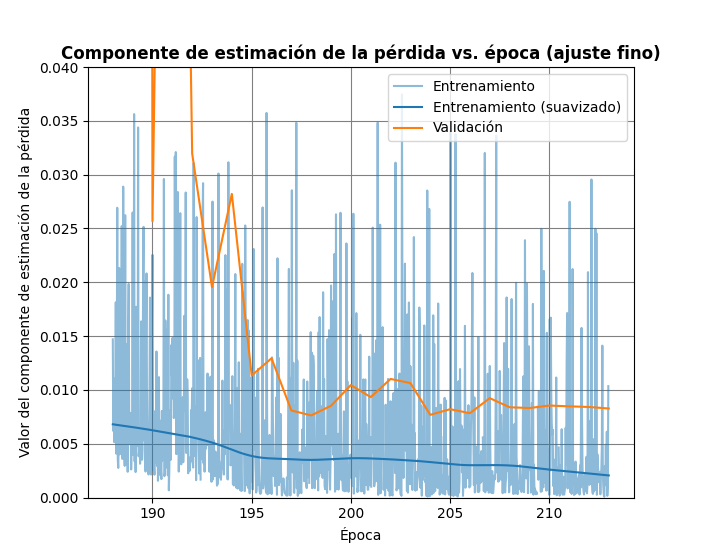
\includegraphics[scale=0.6]{partes/img/loss-estim-stopped.png}
    \caption[Componente de estimación de la pérdida vs. época (ajuste fino) luego de detener el entrenamiento tempranamente.]{Componente de estimación de la pérdida vs. época (ajuste fino) luego de detener el entrenamiento tempranamente. No se observa divergencia en el valor de la pérdida sobre el conjunto de validación.}
    \label{fig:loss-estim-stopped}
\end{figure}

Luego de eliminar la divergencia de la pérdida de validación, se puede proceder a evaluar este modelo contra el modelo original. Como las métricas de utilizadas en la evaluación del método propuesto en \cite{Loquercio2021} evalúan el sistema completo, la única métrica que se puede utilizar para comparar modelos es, exclusivamente, el valor de la función de pérdida a lo largo de un conjunto de datos. Para que esta comparación sea efectiva, lo importante es seleccionar conjuntos de datos representativos de la comparación deseada. Precisamente esto es lo que se utilizó en este trabajo como herramienta de comparación del desempeño de los modelos de interés. El procedimiento y resultados de la evaluación se describe a continuación.

Los modelos a comparar son el modelo original, que destaca en la capacidad de predecir trayectorias sin colisión con \jim{v_{des} = 7} m/s; y el modelo ajustado en este trabajo para predecir trayectorias sin colisión con \jim{v_{des} = 1} m/s. Para ello, se seleccionaron dos conjuntos de datos, el conjunto de datos de validación con trayectorias con \jim{v_{des} = 7} m/s (utilizado en el entrenamiento del modelo original) y el conjunto de datos de validación con las trayectorias con \jim{v_{des} = 1} m/s (el generado en el presente trabajo). La diferencia en los valores de pérdida entre esos modelos y conjuntos de datos, dan una idea del rendimiento relativo de cada uno de los modelos dentro de los escenarios presenciados en el conjunto de datos. La Tabla \ref{table:loss-comparison} compara los valores de pérdida de cada modelo sobre cada conjunto de datos de interés.

\begin{table}[h]
    \centering
    \begin{tabular}{||c | c || c | c ||} 
     \hline
     \textbf{Modelo} & \textbf{Conjunto de datos} & \jim{L_{esp}} & \jim{L_{est}}  \rule{0pt}{2.6ex} \\ [0.4ex] 
     \hline\hline
     Original & Original a 7 m/s & \textbf{1.407} & 0.1069 \\ 
     \hline
     Original & Generado a 1 m/s & \textbf{41.7108} & 0.0842 \\ 
     \hline
     Ajustado & Generado a 1 m/s & \textbf{0.0441}  & 0.0008 \\
     \hline
    \end{tabular}
    \caption[Comparación de los valores de pérdida entre modelo original y ajustado según el conjunto de datos evaluado.]{Comparación de los valores de pérdida entre modelo original y ajustado según el conjunto de datos evaluado. \jim{L_{esp}} es el valor del componente espacial de la pérdida y \jim{L_{est}} es el valor del componente de estimación de la pérdida.}
    \label{table:loss-comparison}
\end{table}

De esta comparación podemos se pueden realizar algunas observaciones relevantes. Primero, el modelo original tiene dificultades en generar trayectorias con las características espaciales de las trayectorias con \jim{v_{des} = 1} m/s, esto tiene sentido pues la diferencia espacial entre moverse a 7 m/s y 1 m/s es bastante alta; esto simplemente confirma la dependencia entre \jim{v_{des}} del experto y el desempeño de la política estudiante a distintas velocidades, tal como se afirma en \cite{Loquercio2021}. Por otro lado, el modelo original logra generalizar la tarea de estimar el costo de ejecución de una trayectoria, los valores del componente de estimación de la pérdida están en el mismo orden tanto para \jim{v_{des} = 7} m/s como para \jim{v_{des} = 1} m/s. 

Segundo, y más relevante para este trabajo, los valores de pérdida del modelo ajustado sobre el conjunto con \jim{v_{des} = 1} m/s, están dos órdenes de magnitud por debajo de los valores del modelo original sobre el conjunto con \jim{v_{des} = 7} m/s; esto puede indicar la presencia de sobre-ajuste (pérdida de capacidad de generalización), sin embargo, este sobre-ajuste no existe al nivel de conjuntos de entrenamiento y de validación, sino que existe al nivel de los conjuntos de datos generados por el experto con distintos valores de \jim{v_{des}}. Para confirmar esta línea de pensamiento, se procede a visualizar una muestra de las trayectorias generadas con \jim{v_{des} = 1} m/s y compararlas con una muestra de las trayectorias generadas con \jim{v_{des} = 7} m/s. Si ambos conjuntos de datos tienen niveles equivalentes de generalización, se debería observar en cada muestra una representación amplia de distintas trayectorias. Si alguna de las dos muestras tiene preferencia por un caso particular de trayectorias con respecto a la otra muestra, entonces esa base de datos tiene menos capacidad de generalización relativamente. De cada base de datos se seleccionaron tres vuelos aleatoriamente, la Figura \ref{fig:7ms-sample} y la Figura \ref{fig:1ms-sample} visualizan las muestras seleccionadas. Cada muestra se visualiza como una vista ``de arriba hacia abajo'' de la nube de puntos del entorno junto con las trayectorias generadas durante el vuelo; el color de las trayectorias interpola entre azul y rojo, mientras más rojo, más costo de ejecución tiene la trayectoria. Este experimento se repitió 10 veces con resultados similares. Para facilitar la visualización de los resultados, solo se muestra un solo experimento.

\begin{figure}[H]
    \centering
    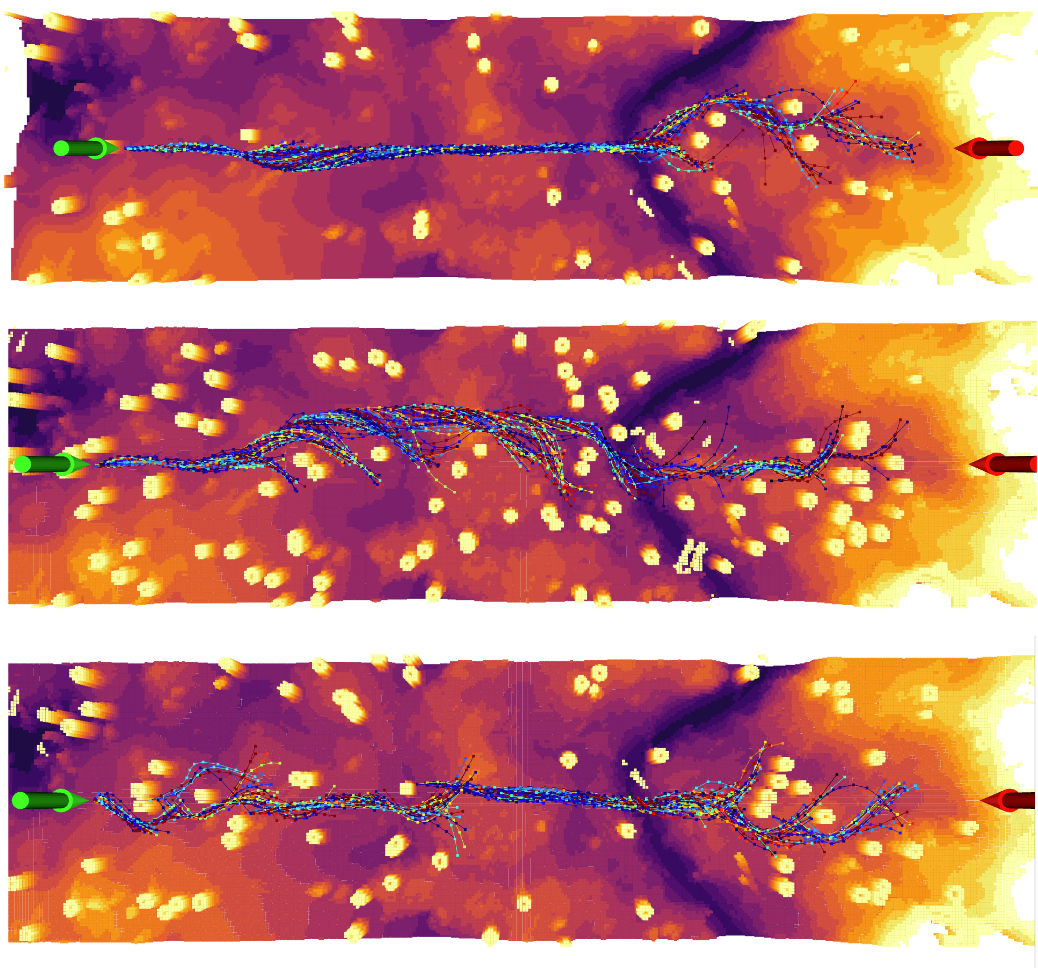
\includegraphics[scale=0.4]{partes/img/7ms-sample.png}
    \caption[Visualización de tres vuelos de la base de datos con \jim{v_{des} = 7} m/s.]{Visualización de tres vuelos de la base de datos con \jim{v_{des} = 7} m/s.}
    \label{fig:7ms-sample}
\end{figure}

\begin{figure}[H]
    \centering
    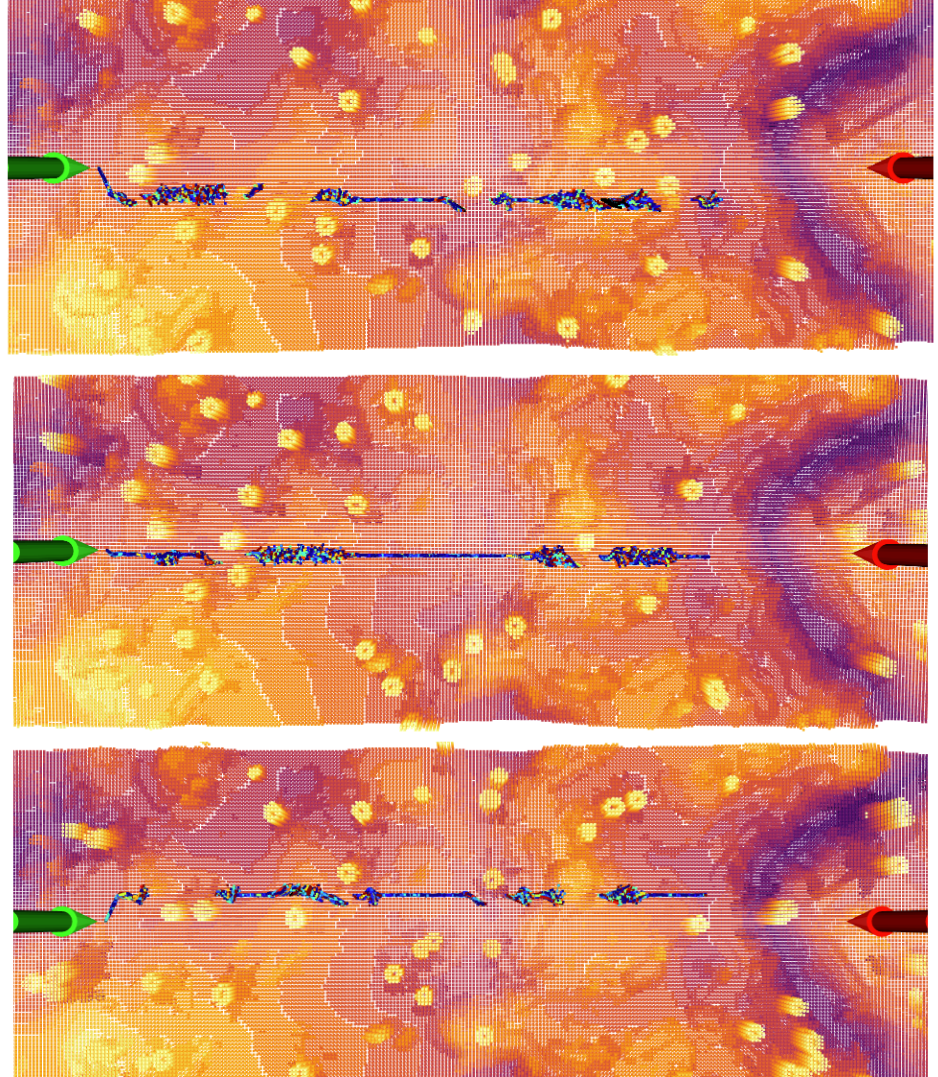
\includegraphics[scale=0.4]{partes/img/1ms-sample.png}
    \caption[Visualización de tres vuelos de la base de datos con \jim{v_{des} = 1} m/s.]{Visualización de tres vuelos de la base de datos con \jim{v_{des} = 1} m/s.}
    \label{fig:1ms-sample}
\end{figure}

A simple vista se observa una clara diferencia, en la base de datos con \jim{v_{des} = 1} m/s, los obstáculos solo se esquivan por uno solo de los flancos del obstáculo, mientras en la base de datos con \jim{v_{des} = 7} m/s se exploran ambos flancos como posibilidades de esquivar el obstáculo. Para cuantificar esta observación, se procedió a contar para cada conjunto de datos, el porcentaje de ejemplos en donde la trayectoria se dirige hacia la izquierda, hacia la derecha y hacia al frente. Para determinar si un ejemplo de la base de datos va hacia a la izquierda, derecha o hacia el frente; se calculan \jim{D_{r}} y \jim{D_{l}} los desplazamientos máximos hacia la derecha y hacia la izquierda respectivamente, con respecto al marco de referencia del cuerpo del QUAV. Luego si \jim{\vert D_{r} - D_{l}\vert < 0.1 } se considera que la trayectoria va hacia el frente, si \jim{D_{r} > D_{l}} se considera que la trayectoria va hacia la derecha y si \jim{D_{r} < D_{l}} se considera que la trayectoria va hacia la izquierda. Solo se consideran los ejemplos en donde exista un obstáculo visible a 5m de distancia. La Tabla \ref{table:flank-count} muestra los resultados de este conteo. 

\begin{table}[h]
    \centering
    \begin{tabular}{||c | c | c | c | c ||} 
     \hline
     \textbf{Conjunto de datos} & \jim{P_{left}} & \jim{P_{right}} & \jim{P_{str}} & \jim{N_{samples}} \rule{0pt}{2.6ex} \\ [0.4ex] 
     \hline\hline
     \jim{v_{des} = 7} m/s & 51.3\% & 44.1\% & 4.5\% & 5517 \\ 
     \hline
     \jim{v_{des} = 1} m/s & 40.6\% & 35.1\% & 24.3\% & 18244 \\ 
     \hline
    \end{tabular}
    \caption[Distribución de ejemplos en cada conjunto de datos según hacia donde se dirige la trayectoria.]{Distribución de ejemplos en cada conjunto de datos según hacia donde se dirige la trayectoria. \jim{P_{left}} es el porcentaje de ejemplos en donde la trayectoria se dirige hacia la izquierda, \jim{P_{right}} es el porcentaje de ejemplos en donde la trayectoria se dirige hacia la derecha, \jim{P_{str}} es el porcentaje de ejemplos en donde la trayectoria se dirige hacia el frente y \jim{N_{samples}} es el número de ejemplos en el conjunto de datos.}
    \label{table:flank-count}
\end{table}

De los resultados presentados en la Tabla \ref{table:flank-count} podemos realizar varias observaciones. Primero ambos conjuntos de datos tienen un desbalance entre \jim{P_{left}} y \jim{P_{right}}, con \jim{P_{left}} dominando por 5\%. Segundo, el conjunto de datos con \jim{v_{des} = 1} m/s contiene un número mucho mayor de trayectorias que se dirigen hacia el frente, con un 24.3\% de los ejemplos, mientras que el conjunto de datos con \jim{v_{des} = 7} m/s solo tiene un 4.5\% de los ejemplos. Tercero, el conjunto de datos con \jim{v_{des} = 1} m/s tiene un 230\% más ejemplos que el conjunto de datos con \jim{v_{des} = 7} m/s, esto probablemente como consecuencia de recorrer una distancia menor en promedio por trayectoria (por la menor rapidez de desplazamiento). 

Como la decisión de esquivar un obstáculo en el plano \jim{xy} se reduce a esquivar por el flanco izquierdo o por el flanco derecho del obstáculo (pues seguir hacia el frente implica colisión), el desbalance entre \jim{P_{left}} y \jim{P_{right}} es el factor mas relevante en la diferencia de capacidad de generalización entre los conjuntos de datos. Este factor es además acentuado en el conjunto con \jim{v_{des} = 1} m/s por el mayor número de ejemplos que se dirigen hacia el frente, y por el mayor número de ejemplos en general; haciendo que el 5\% de desbalance entre \jim{P_{left}} y \jim{P_{right}} sea mucho más relevante. Es por esto que el modelo ajustado va a tener una preferencia a esquivar obstáculos por el flanco izquierdo. En otras palabras, existe un desbalance de las modas de la distribución \jim{P}\footnote{La distribución \jim{P} se describe en la Ecuación \ref{eq:aoa-expert-P}} en la base de datos con \jim{v_{des} = 1} m/s que no existe significativamente en en la base de datos con \jim{v_{des} = 7} m/s. Este desbalance hace que el proceso de refinamiento fino produzca un efecto de sobre-ajuste con respecto al rendimiento de la política publicada en \cite{Loquercio2021}. El modelo se ajusta demasiado a los ejemplos de la base datos con \jim{v_{des} = 1} m/s, en donde existe una preferencia significativa a esquivar obstáculos por el flanco izquierdo, potencialmente reduciendo su capacidad multi-modal al momento de generar trayectorias.

Un posible origen de este problema, es que la poca longitud de las trayectorias generadas para \jim{v_{des} = 1} m/s no permite que el experto genere trayectorias que consideren todas las modas de la distribución \jim{P} con un valor de costo bajo. Cuando el experto selecciona las mejores tres trayectorias, algunas de las trayectorias que consideran las modas de \jim{P} se descartan, produciendo el desbalance. Otra posible razón puede ser que el planificador de trayectorias globales que genera \jim{\tau_{ref}} no permita la exploración de dichas trayectorias, principalmente por planificar trayectorias triviales en donde se navegue mayoritariamente sin encontrar obstáculos. 

Una posible solución para este problema es modificar el entorno de simulación para que la configuración de los obstáculos permita que el experto considere las modas de \jim{P} con alto valor de costo, por ejemplo, incrementando la densidad de los obstáculos y reduciendo sus dimensiones. Otra posible solución es modificar los parámetros del planificador de trayectorias globales de forma que la ejecución de \jim{\tau_{ref}} fomente la exploración de obstáculos en donde se generen muestras que representen el carácter multi-modal de \jim{P}, por ejemplo, intencionalmente dirigiéndose hacia la cercanía de grupos de obstáculos. Alternativamente se pueden ejecutar las predicciones de la red en lugar de seguir una \jim{\tau_{ref}} planificada globalmente, y en su lugar utilizar una \jim{\tau_{ref}} que simplemente sea el camino en línea recta desde el punto de despegue hasta la meta; esto potencialmente va a incrementar la exploración de obstáculos en donde se generen muestras que representen múltiples modas de \jim{P}.

Dicho esto, por limitaciones del tiempo de desarrollo, y recomendaciones por parte del equipo de ACSL, en este trabajo no se soluciona el problema descrito anteriormente. Esto significa que la política estudiante utilizada en este trabajo sufre las consecuencias del sobre-ajuste ocasionado por el desbalance de modas en la base de datos con \jim{v_{des} = 1} m/s, esto puede ocasionar que la política de evasión de obstáculos tenga una preferencia fuerte en esquivar obstáculos de una forma en particular. En las siguientes secciones se observa que efectivamente, la política de evasión de obstáculos tiene una fuerte preferencia a esquivar obstáculos por el flanco izquierdo, así como también, que este comportamiento hace que la ejecución en entornos no triviales termine en potenciales colisiones.

\section{Resultados de la política de evasión de obstáculos}

\label{sec:results-flights}

\subsection{Vuelos en entorno simulación}

\label{sec:results-AirSim}

En esta sección se describen las configuraciones de los vuelos realizados en el entorno de simulación AirSim \cite{shah2018airsim}, así como también sus resultados y comportamientos observados. Es importante recordar que por motivos de validación del concepto por parte de ACSL, la ejecución de la evasión de obstáculos está limitada al plano \jim{xy} del marco de referencia del cuerpo del QUAV.

La primera configuración de obstáculos utilizada es una configuración simple con un solo obstáculo en la línea directa de visión del QUAV, un diagrama de la configuración se muestra en la Figura \ref{fig:config-1-single}. En el diagrama se muestran dos vistas, la frontal (plano \jim{yz}) a partir desde el punto de despegue y la vista de arriba hacia abajo (plano \jim{xy}).

\begin{figure}[H]
    \centering
    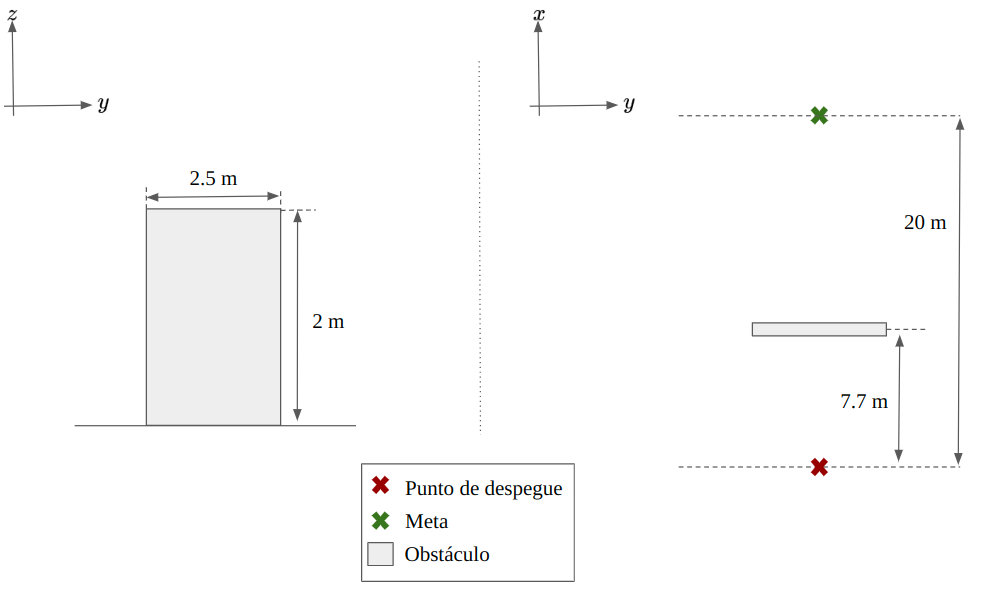
\includegraphics[scale=0.35]{partes/img/config-1-single.png}
    \caption[Primera configuración de obstáculos dentro del entorno de AirSim.]{Primera configuración de obstáculos dentro del entorno de AirSim. Obstáculo simple.}
    \label{fig:config-1-single}
\end{figure}

El comportamiento del algoritmo se mostró capaz de evadir el obstáculo de forma robusta, en concreto, de 10 vuelos ejecutados, 10 resultaron en vuelos sin colisión. La Figura \ref{fig:single-graph-4} muestra una visualización desde arriba hacia abajo de los caminos resultantes de seguir las trayectorias generadas por el algoritmo para cuatro vuelos. Todos los vuelos realizados en esta configuración muestran un comportamiento similar a lo que se observa en la Figura \ref{fig:single-graph-4}, esto es, esquivar el obstáculo hacia la dirección \jim{-y_B}\footnote[1]{Donde \jim{B} es el marco de referencia del cuerpo del QUAV.} y dirigirse hacia la meta una vez no es visible el obstáculo.

\begin{figure}[H]
    \centering
    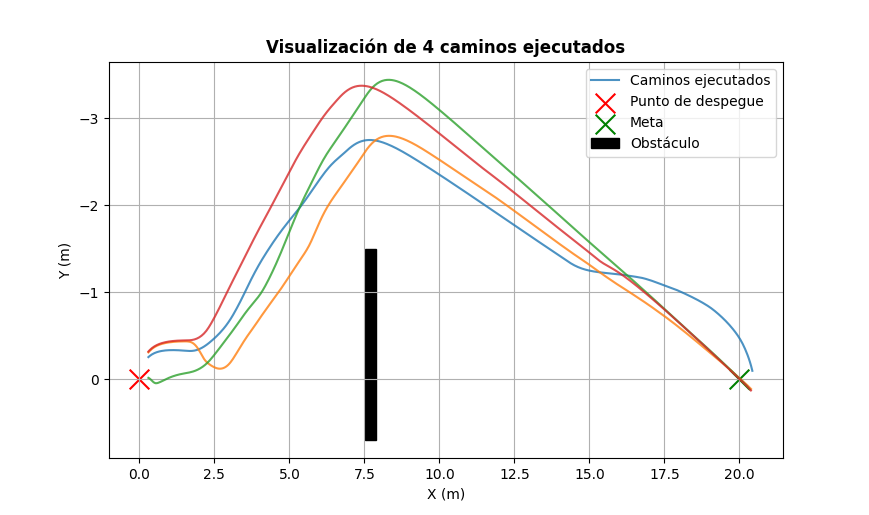
\includegraphics[scale=0.65]{partes/img/sim-single-panel-graph-4.png}
    \caption[Visualización simultánea de cuatro caminos ejecutados dentro de la primera configuración de obstáculos en entorno de simulación.]{Visualización simultánea de cuatro caminos ejecutados dentro de la primera configuración de obstáculos en entorno de simulación. De 10 vuelos ejecutados dentro de esta configuración, 10 resultaron sin colisión.}
    \label{fig:single-graph-4}
\end{figure}

La diferencia más marcada entre vuelos en esta configuración es la desviación máxima del camino ejecutado con respecto al camino directo entre el punto de despegue y la meta, la Figura \ref{fig:single-max-deviation} muestra un diagrama de caja de la desviación máxima de los caminos ejecutados en esta configuración. La desviación máxima promedio de los caminos ejecutados en esta configuración es cerca de 3.1 metros, con una desviación máxima de cerca de 3.45 metros y una desviación mínima de cerca de 2.75 metros.

\begin{figure}[H]
    \centering
    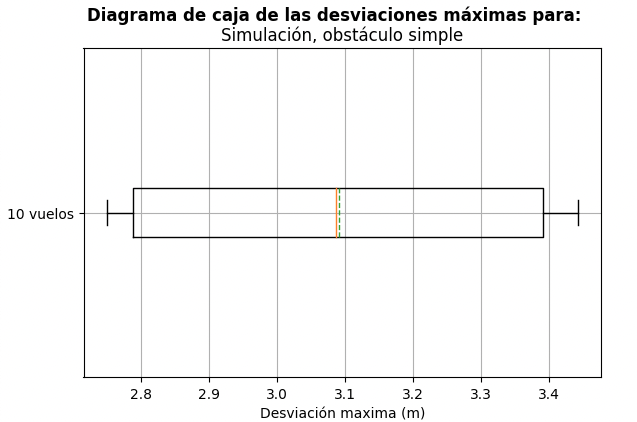
\includegraphics[scale=0.55]{partes/img/sim-single-panel-box.png}
    \caption[Diagrama de caja de la desviación máxima de los caminos ejecutados en la primera configuración de obstáculos en entorno de simulación.]{Diagrama de caja de la desviación máxima de los caminos ejecutados en la primera configuración de obstáculos en entorno de simulación.}
    \label{fig:single-max-deviation}
\end{figure}

La siguiente configuración utilizada es una configuración similar a la anterior pero con un obstáculo adicional también en la misma línea de visión del QUAV. La Figura \ref{fig:config-2-double} muestra el diagrama de la segunda configuración.

\begin{figure}[H]
    \centering
    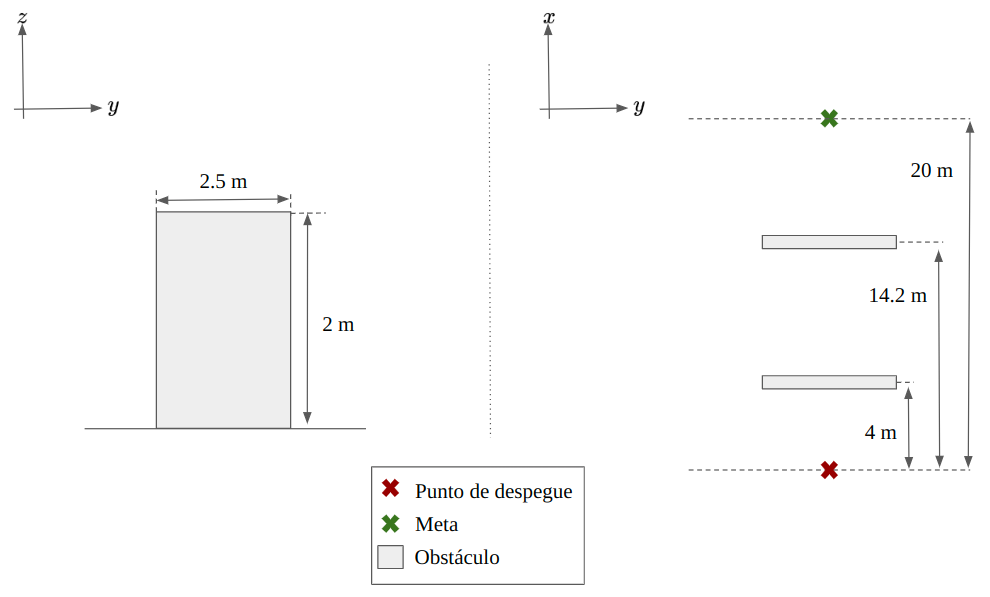
\includegraphics[scale=0.35]{partes/img/config-2-double.png}
    \caption[Segunda configuración de obstáculos dentro del entorno de AirSim.]{Segunda configuración de obstáculos dentro del entorno de AirSim. Dos obstáculos consecutivos en la línea de visión del QUAV.}
    \label{fig:config-2-double}
\end{figure}

Tal como en la configuración anterior, el comportamiento de algoritmo fue estable, de 10 vuelos ejecutados, 10 resultaron en vuelos sin colisión. La Figura \ref{fig:double-graph-4} muestra una visualización desde arriba hacia abajo de caminos resultantes de seguir las trayectorias generadas por el algoritmo para cuatro vuelos. Todos los vuelos realizados en esta configuración muestran un comportamiento similar a lo que se observa en la Figura \ref{fig:double-graph-4}.

\begin{figure}[H]
    \centering
    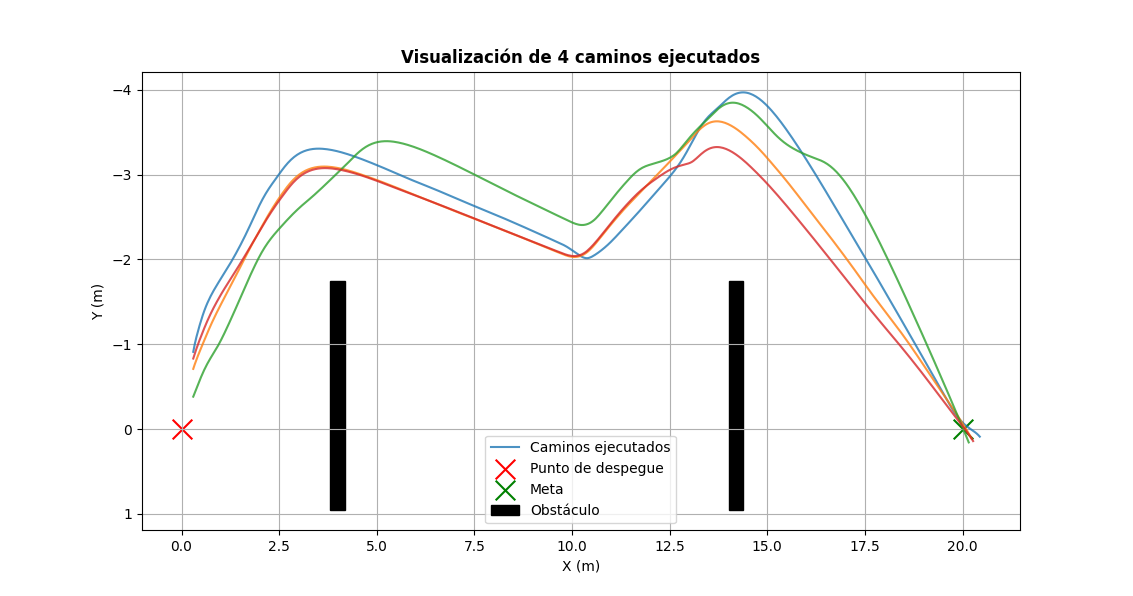
\includegraphics[scale=0.5]{partes/img/sim-double-panel-graph-4.png}
    \caption[Visualización simultánea de 4 caminos ejecutados dentro de la segunda configuración de obstáculos en entorno de simulación.]{Visualización simultánea de 4 caminos ejecutados dentro de la segunda configuración de obstáculos en entorno de simulación. De 10 vuelos ejecutados dentro de esta configuración, 10 resultaron sin colisión.}
    \label{fig:double-graph-4}
\end{figure}

En lo que respecta a la desviación máxima de los caminos ejecutados en esta configuración, la Figura \ref{fig:double-max-deviation} muestra un diagrama de caja de la desviación máxima de los caminos ejecutados. La desviación máxima promedio de los caminos ejecutados en esta configuración es cerca de 3.7 metros, con una desviación máxima de cerca de 4 metros y una desviación mínima de cerca de 3.3 metros. Estos resultados muestran como la maniobra para esquivar el segundo obstáculo incrementa la desviación máxima de los caminos ejecutados.

\begin{figure}[H]
    \centering
    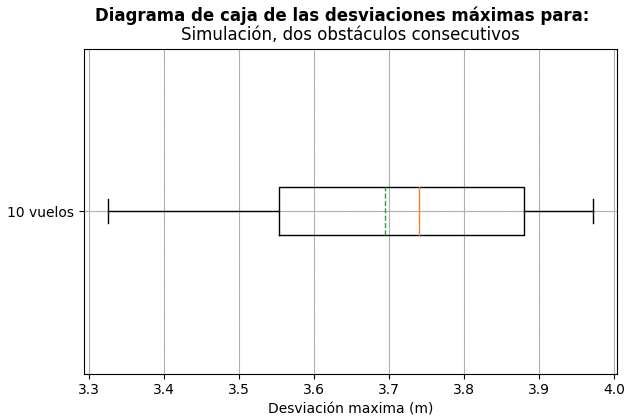
\includegraphics[scale=0.55]{partes/img/sim-double-panel-box.png}
    \caption[Diagrama de caja de la desviación máxima de los caminos ejecutados en la segunda configuración de obstáculos en entorno de simulación.]{Diagrama de caja de la desviación máxima de los caminos ejecutados en la segunda configuración de obstáculos en entorno de simulación.}
    \label{fig:double-max-deviation}
\end{figure}

Es interesante resaltar, que en los vuelos dentro de la segunda configuración, se confirma el funcionamiento del mecanismo que desactiva la inferencia cuando no hay obstáculos visibles. Para visualizar esto, se desarrolló una visualización 3D que permite visualizar la ejecución del algoritmo incluyendo la información sensorial de profundidad y las trayectorias generadas. En esta visualización se muestra:

\begin{itemize}
    \item La nube de puntos del entorno percibido por las cámaras estereoscópicas del QUAV, el color de los puntos indica la profundidad con respecto al sistema de cámaras, mientras más rojo más cerca y mientras más azul más lejos.
    \item El camino ejecutado por el QUAV, que se muestra como una curva de color blanco.
    \item La trayectoria más reciente generada por la política estudiante, que se muestra como una curva de color verde que comienza en la posición en donde se realizo la inferencia.
    \item El radio de colisión del QUAV, que se muestra como una circunferencia de color azul alrededor de la posición del QUAV. Si un obstáculo entra dentro de esta circunferencia se considera una colisión.
    \item La dirección del encabezamiento del QUAV, que se muestra como una línea roja que parte de la posición del QUAV.
    \item Las posiciones de despegue y de meta, que se muestran como un circulo rojo y verde respectivamente.
    \item El camino directo entre el punto de despegue y la meta.
    \item La orientación tridimensional del entorno, que se muestra como 3 flechas; una azul que representa la dirección del eje \jim{z}, una verde que representa la dirección del eje \jim{y} y una roja que representa la dirección del eje \jim{x}. Es importante mencionar que debido a limitaciones del programa de visualización, la dirección del eje \jim{y} se encuentra invertida con respecto al resto de visualizaciones en este capítulo.
\end{itemize}

La Figura \ref{fig:depth-dual-panel-1}, la Figura \ref{fig:depth-dual-panel-2} y la Figura \ref{fig:depth-dual-panel-3} muestran capturas consecutivas de la visualización 3D de un vuelo dentro de la segunda configuración, desde una perspectiva de arriba hacia abajo. En estas figuras podemos observar como solo se generan trayectorias cuando hay un obstáculo cerca en el campo de visión del QUAV.

\begin{figure}[H]
    \centering
    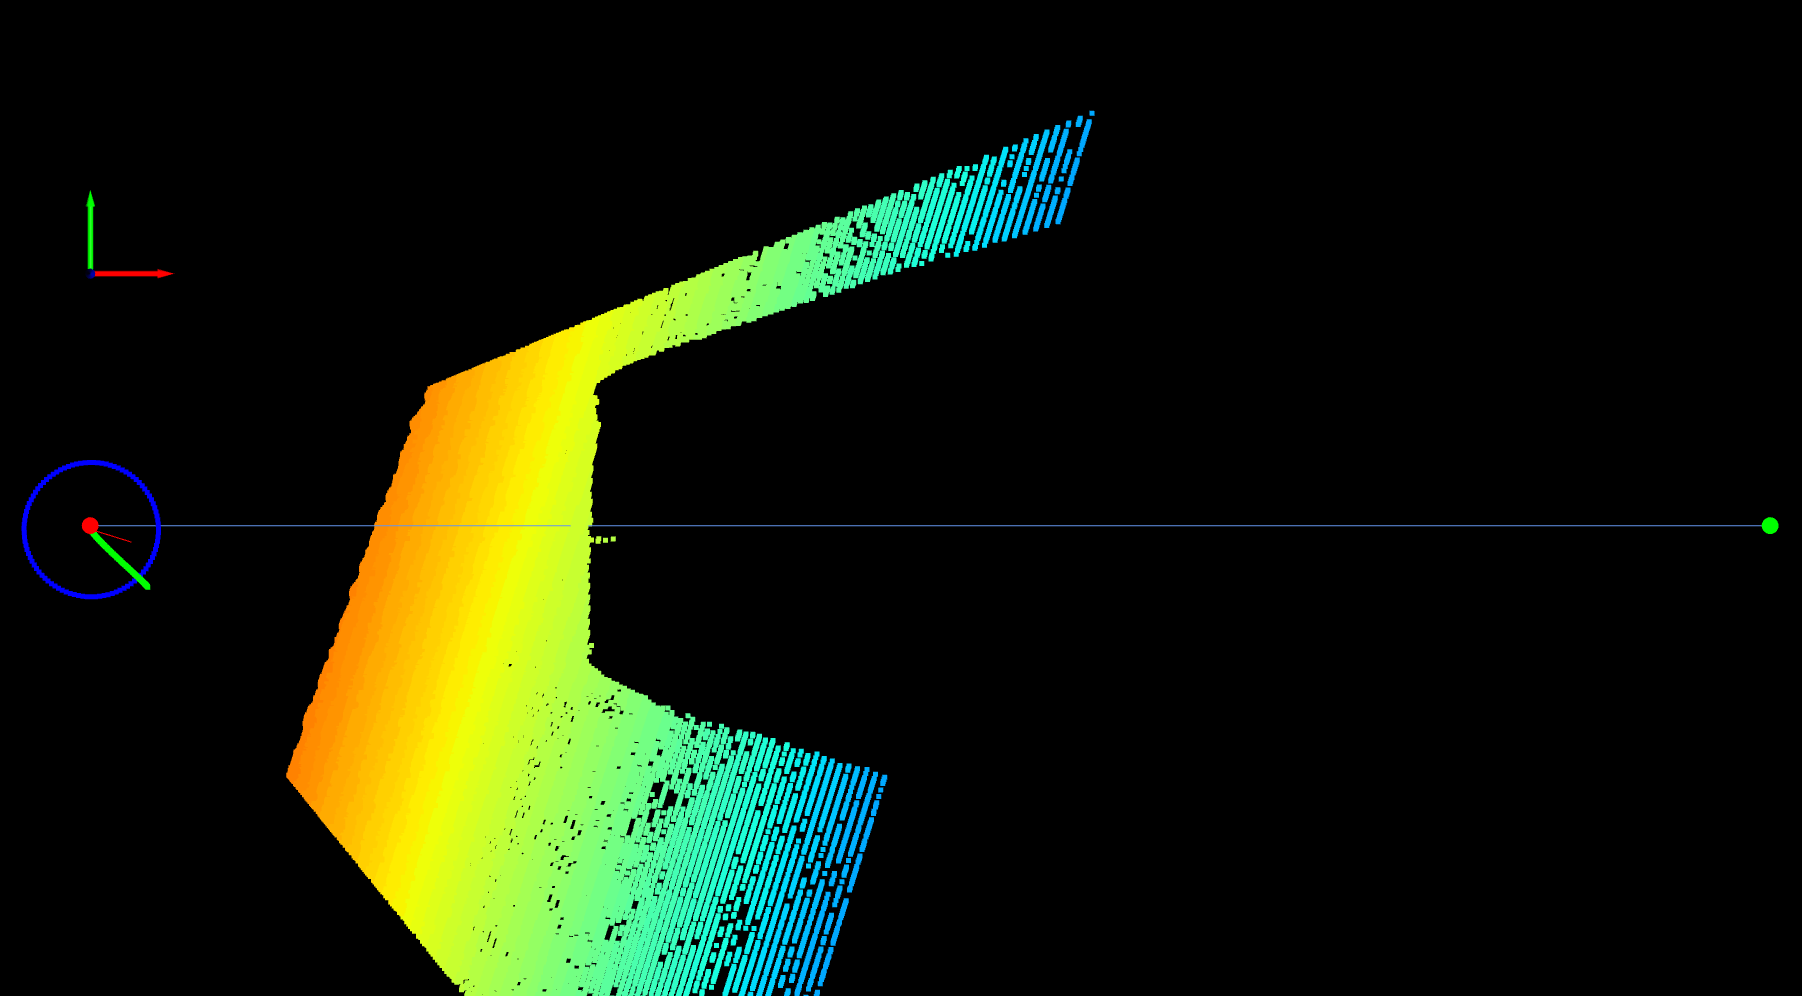
\includegraphics[scale=0.225]{partes/img/depth-dual-panel-1-first-obs.png}
    \caption[Visualización del funcionamiento del mecanismo que desactiva la inferencia cuando no hay obstáculos visibles. Inferencia activada, el primer obstáculo está en el campo de visión.]{Visualización del funcionamiento del mecanismo que desactiva la inferencia cuando no hay obstáculos visibles. Inferencia activada, el primer obstáculo está en el campo de visión.}
    \label{fig:depth-dual-panel-1}
\end{figure}

\begin{figure}[H]
    \centering
    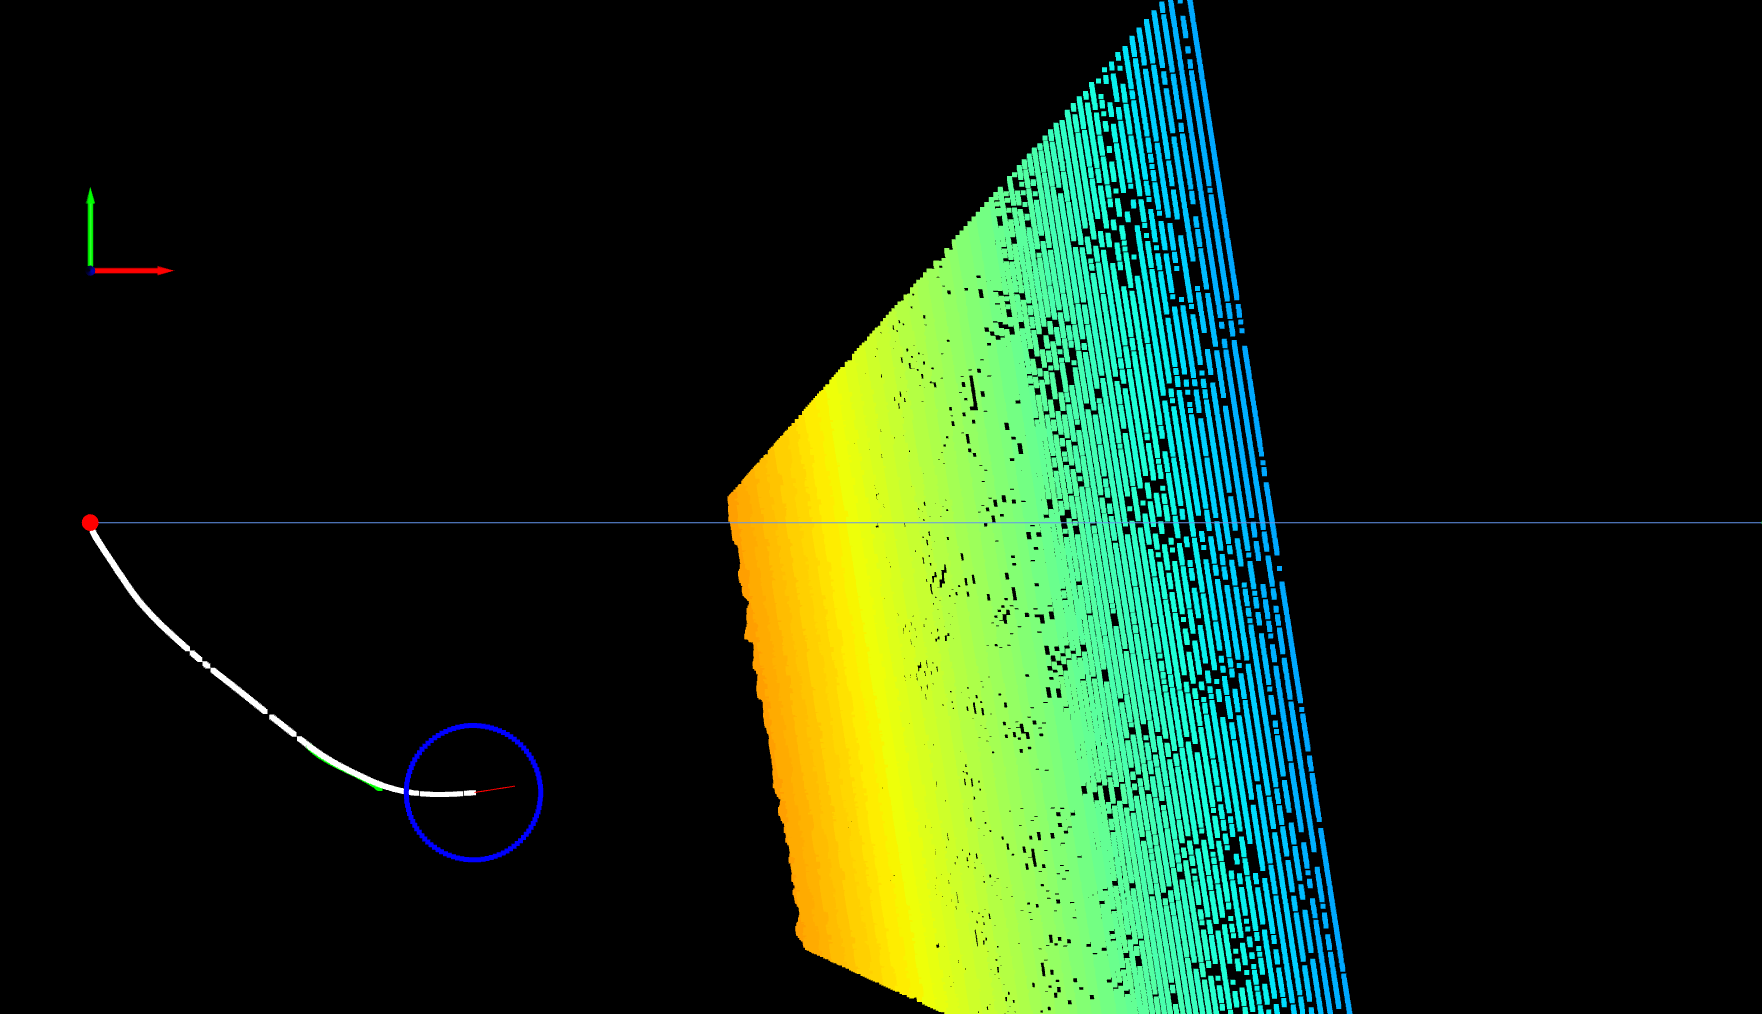
\includegraphics[scale=0.225]{partes/img/depth-dual-panel-2-no-obs.png}
    \caption[Visualización del funcionamiento del mecanismo que desactiva la inferencia cuando no hay obstáculos visibles. Inferencia desactivada, no hay obstáculo visible en campo de visión, navegando en dirección a la meta.]{Visualización del funcionamiento del mecanismo que desactiva la inferencia cuando no hay obstáculos visibles. Inferencia desactivada, no hay obstáculo visible en campo de visión, navegando en dirección a la meta.}
    \label{fig:depth-dual-panel-2}
\end{figure}

\begin{figure}[H]
    \centering
    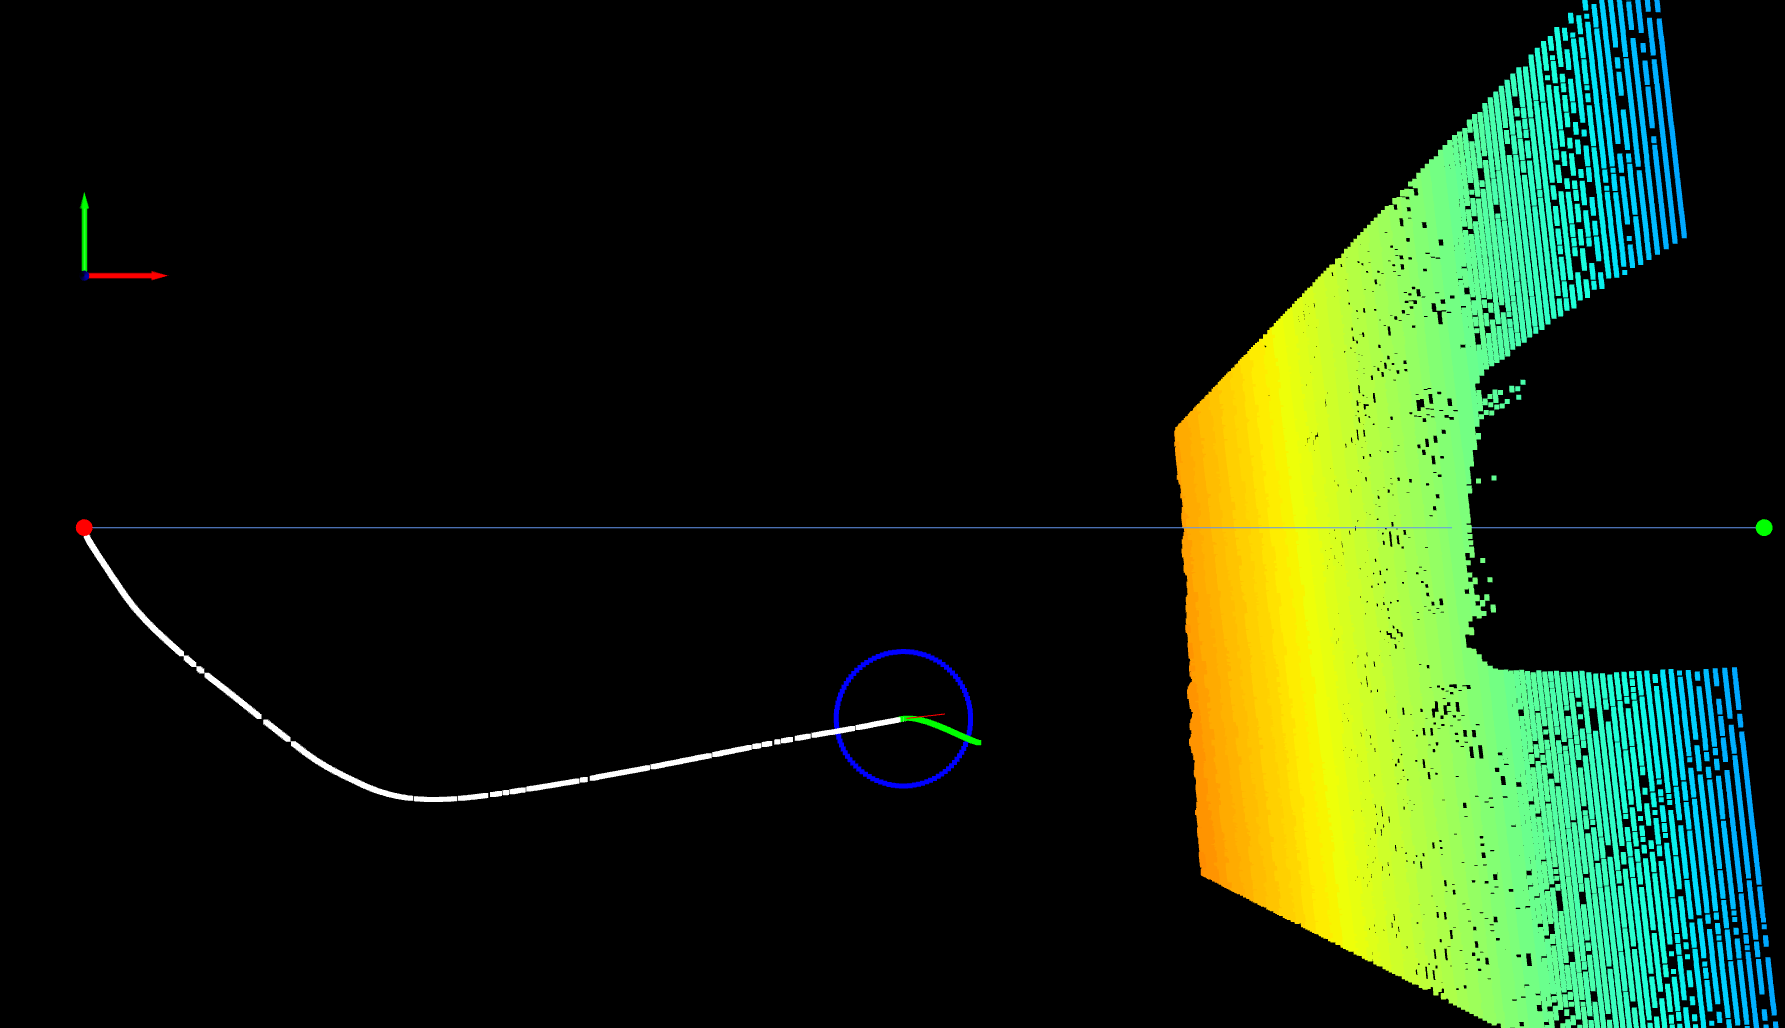
\includegraphics[scale=0.225]{partes/img/depth-dual-panel-3-second-obs.png}
    \caption[Visualización del funcionamiento del mecanismo que desactiva la inferencia cuando no hay obstáculos visibles. Inferencia activada, el segundo obstáculo está en el campo de visión.]{Visualización del funcionamiento del mecanismo que desactiva la inferencia cuando no hay obstáculos visibles. Inferencia activada, el segundo obstáculo está en el campo de visión.}
    \label{fig:depth-dual-panel-3}
\end{figure}

Durante todas las pruebas descritas anteriormente, se observó que la política de evasión de obstáculos tiene una preferencia certera a esquivar obstáculos en la dirección \jim{-y_B}, para evaluar este comportamiento el siguiente conjunto de pruebas utiliza una configuración que coloca un obstáculo adicional hacia esa dirección. La Figura \ref{fig:config-3-parallel} muestra la tercera configuración utilizada, que consiste de dos obstáculos simples paralelos entre si con una separación de 2 metros.

\begin{figure}[H]
    \centering
    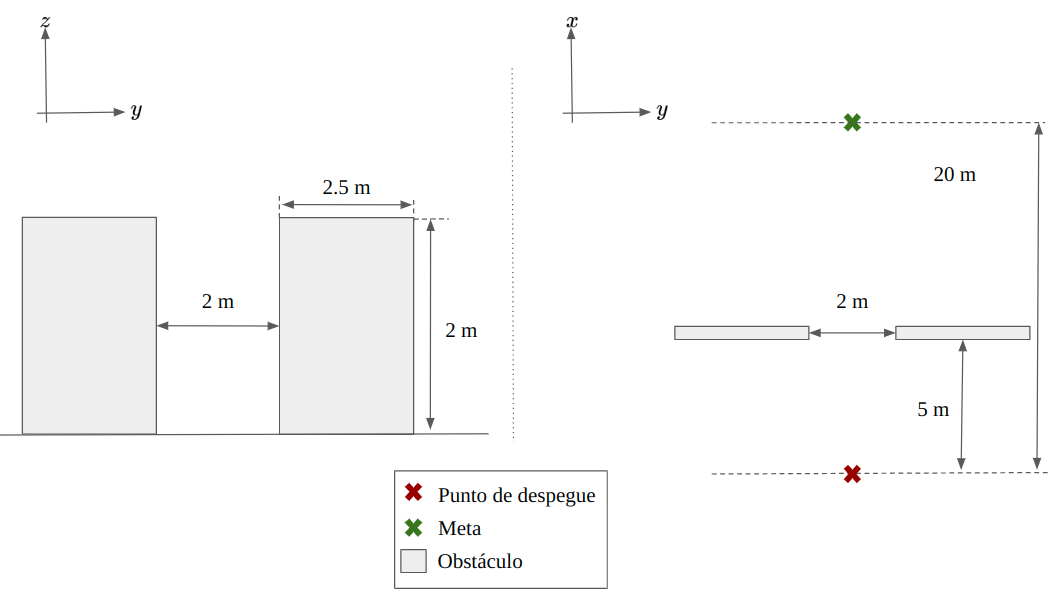
\includegraphics[scale=0.35]{partes/img/config-3-parallel.png}
    \caption[Tercera configuración de obstáculos dentro del entorno de AirSim.]{Tercera configuración de obstáculos dentro del entorno de AirSim. Dos obstáculos paralelos con una separación de 2 metros.}
    \label{fig:config-3-parallel}
\end{figure}

Incluso con la presencia de un obstáculo adicional en la dirección \jim{-y_B}, la política de evasión de obstáculos en todas las pruebas realizadas generó trayectorias dirigidas hacia \jim{-y_B}, lo cual produjo colisiones frecuentes, de 10 vuelos ejecutados, 2 fueron sin colisión. La Figura \ref{fig:depth-parallel-1}, la Figura \ref{fig:depth-parallel-2},  la Figura \ref{fig:depth-parallel-4} y la Figura \ref{fig:depth-parallel-5} muestran una secuencia consecutiva de capturas de la visualización 3D de un vuelo que resultó en colisión. Tal como se aprecia en las figuras, mientras ambos obstáculos son visibles en el campo de visión del QUAV, la trayectoria se dirige al espacio entre ambos obstáculos, con un comportamiento que parece guiar al QUAV a una ejecución sin colisiones; sin embargo, en el momento que solo un de los dos obstáculo es visible, en lugar de continuar dirigiéndose hacia el espacio entre ambos obstáculos, la política intenta corregir la trayectoria para esquivar por el flanco en dirección \jim{-y_B} relativo al obstáculo, lo cual produce una colisión. 

\begin{figure}[H]
    \centering
    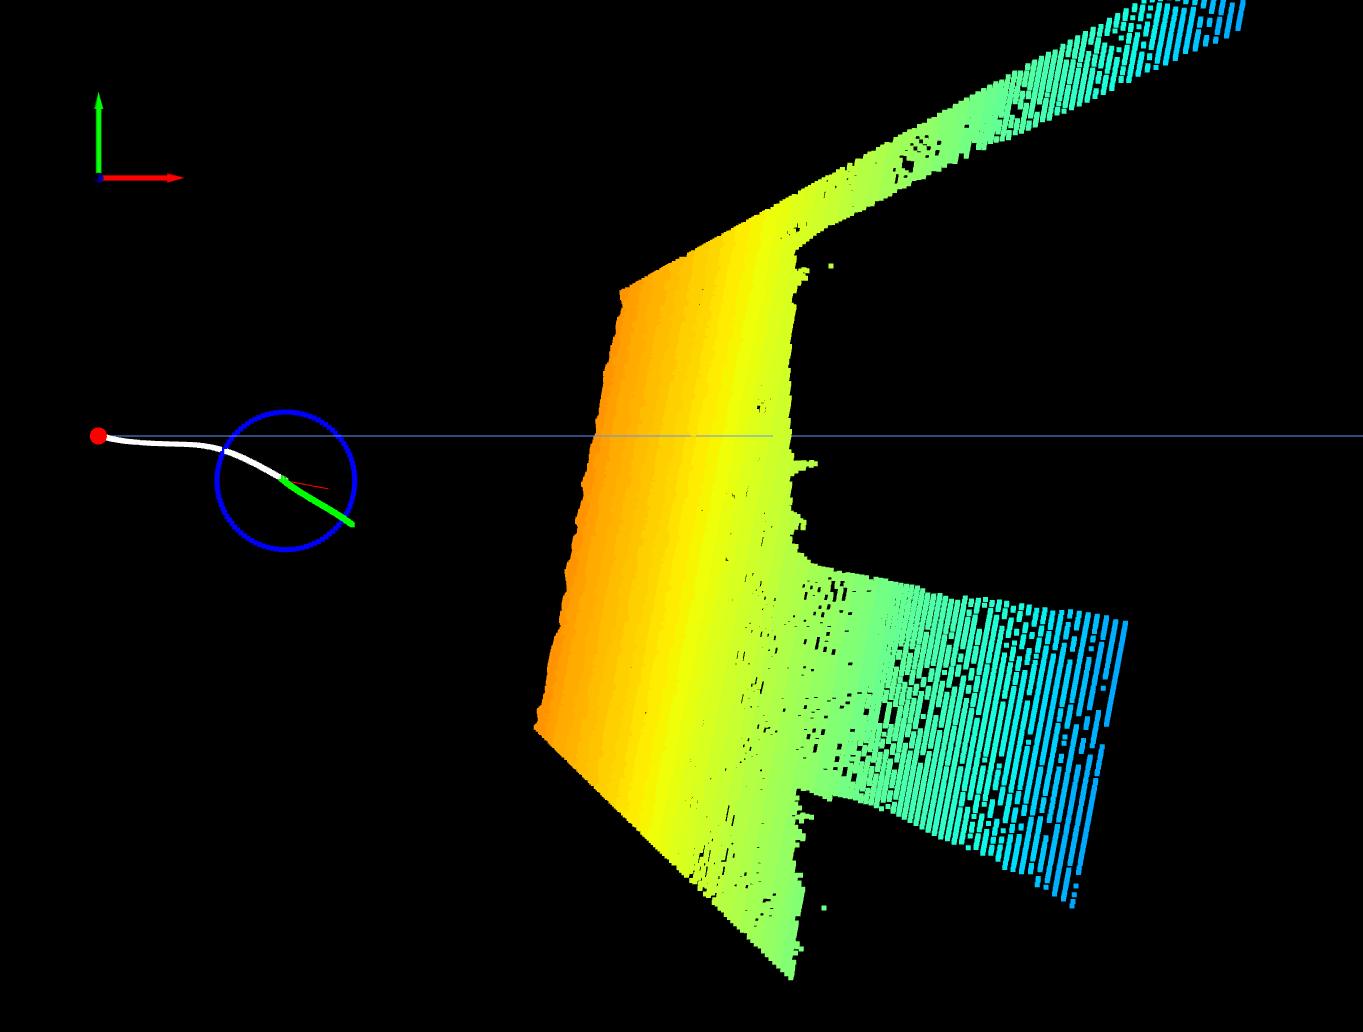
\includegraphics[scale=0.3]{partes/img/depth-parallel-1-topdown.png}
    \caption[Visualización 3D de un vuelo en la tercera configuración de obstáculos (1). Vista de arriba hacia abajo.]{Visualización 3D de un vuelo en la tercera configuración de obstáculos (1). Vista de arriba hacia abajo. Ambos obstáculos están dentro del campo de visión, las trayectorias generadas se dirigen hacia el espacio entre los obstáculos.}
    \label{fig:depth-parallel-1}
\end{figure}

\begin{figure}[H]
    \centering
    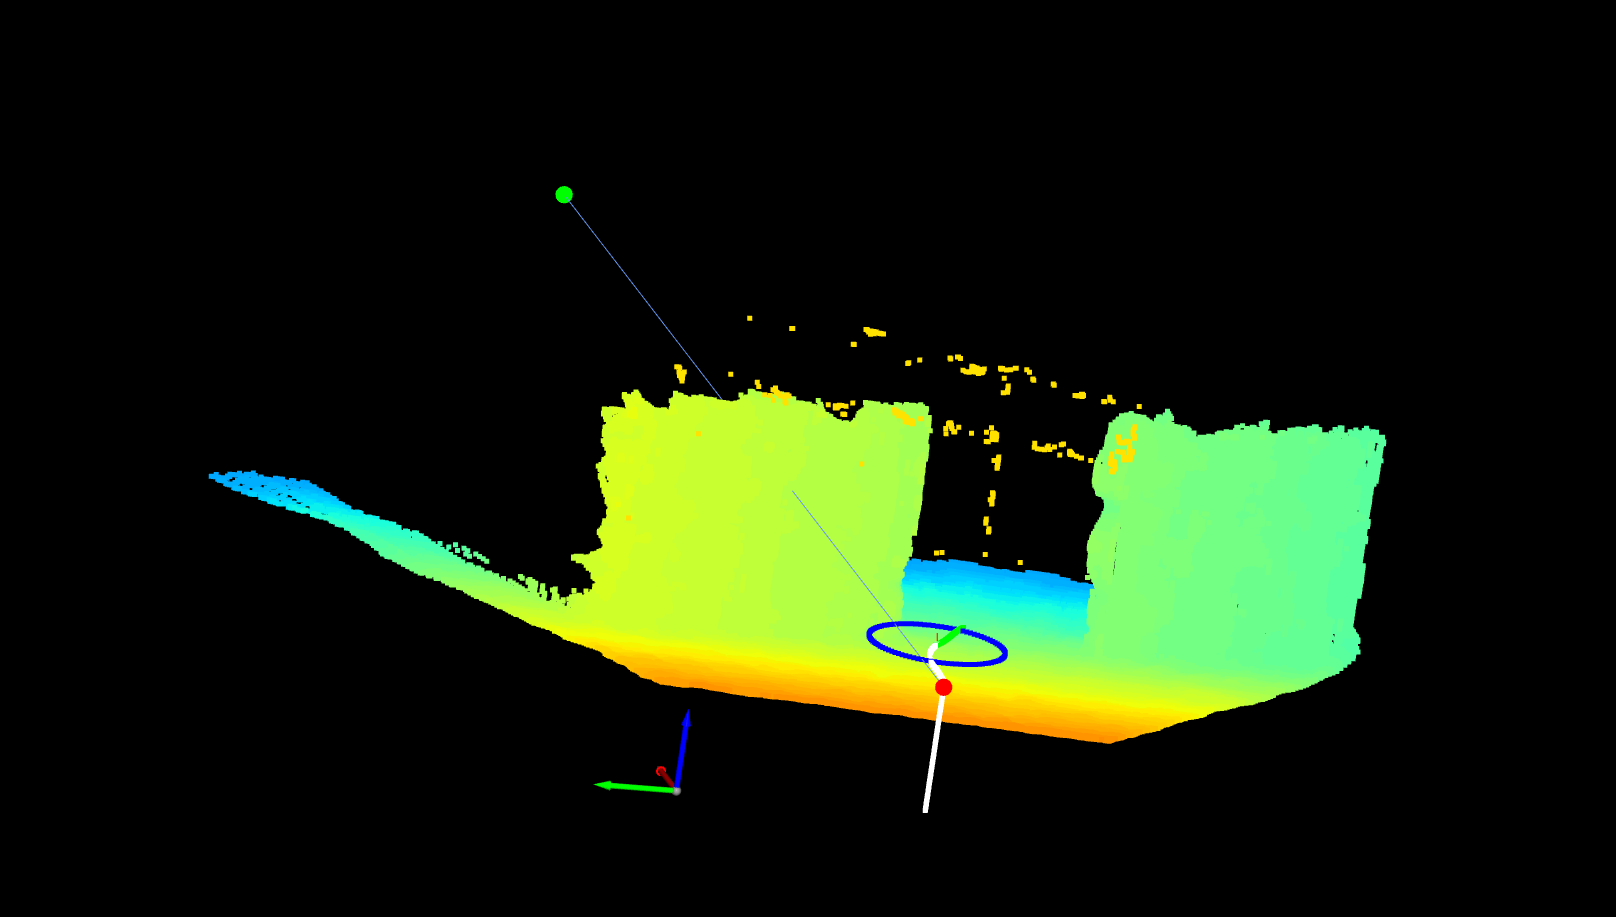
\includegraphics[scale=0.25]{partes/img/depth-parallel-2-front.png}
    \caption[Visualización 3D de un vuelo en la tercera configuración de obstáculos (2). Vista frontal.]{Visualización 3D de un vuelo en la tercera configuración de obstáculos (2). Vista frontal. Ambos obstáculos están dentro del campo de visión, las trayectorias generadas se dirigen hacia el espacio entre los obstáculos.}
    \label{fig:depth-parallel-2}
\end{figure}

\begin{figure}[H]
    \centering
    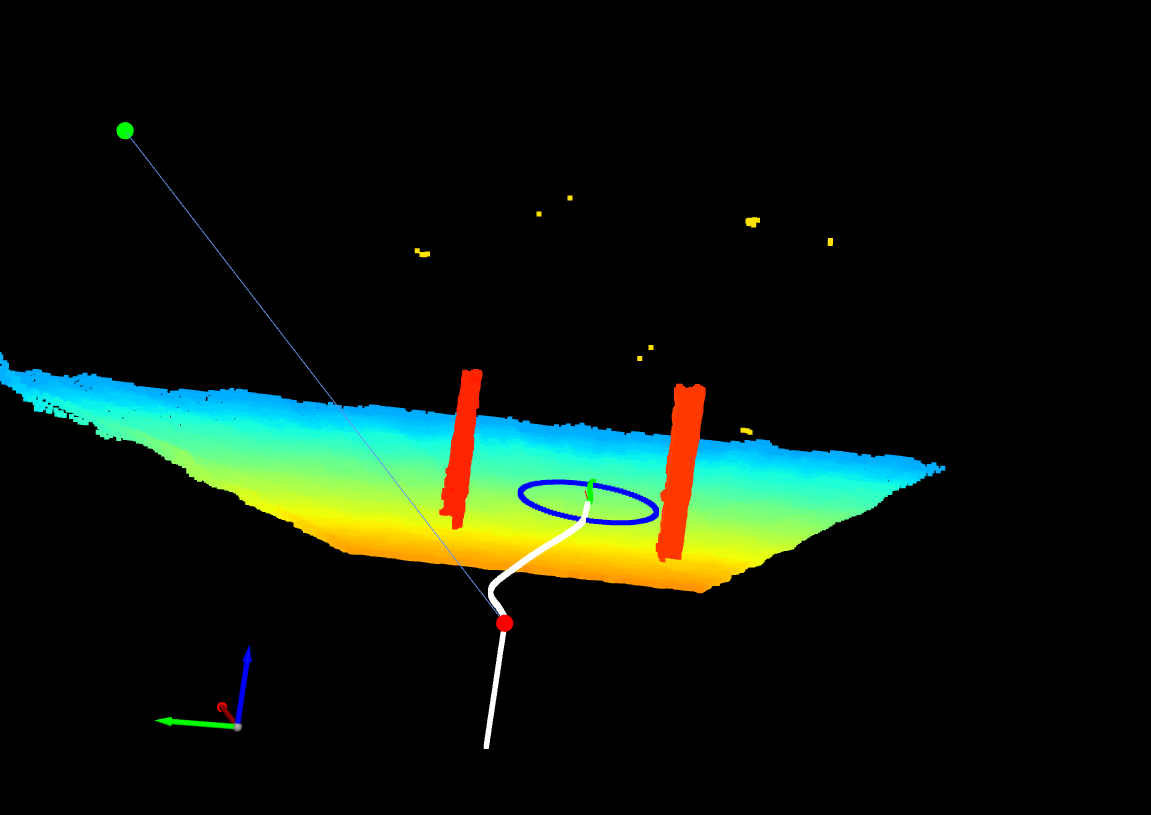
\includegraphics[scale=0.32]{partes/img/depth-parallel-4-front-red.png}
    \caption[Visualización 3D de un vuelo en la tercera configuración de obstáculos (3). Vista frontal. Navegando entre el espacio entre los obstáculos.]{Visualización 3D de un vuelo en la tercera configuración de obstáculos (3). Vista frontal. Navegando entre el espacio entre los obstáculos. Ambos obstáculos están dentro del campo de visión, las trayectorias generadas se dirigen hacia el espacio entre los obstáculos.}
    \label{fig:depth-parallel-4}
\end{figure}

\begin{figure}[H]
    \centering
    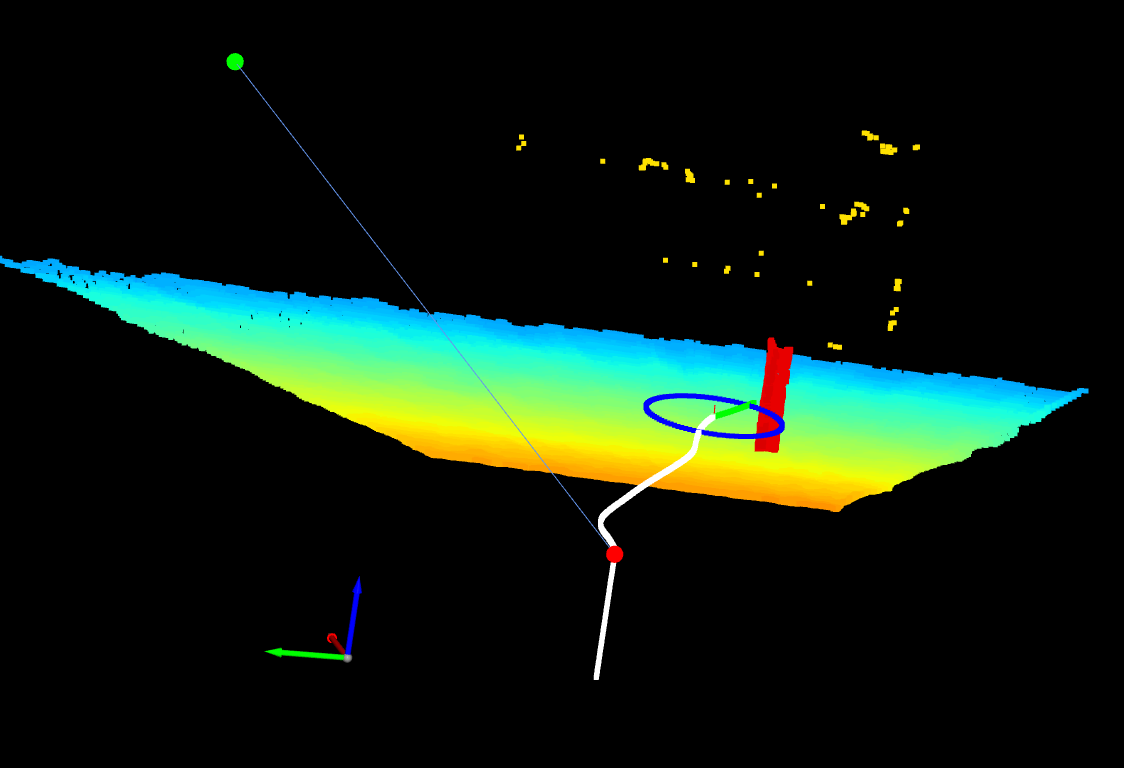
\includegraphics[scale=0.32]{partes/img/depth-parallel-5-front-collision.png}
    \caption[Visualización 3D de un vuelo en la tercera configuración de obstáculos (4). Vista frontal. Colisión.]{Visualización 3D de un vuelo en la tercera configuración de obstáculos (4). Vista frontal. En el momento que uno de los dos obstáculos desaparece del campo de visión, en lugar de continuar dirigiéndose hacia el espacio entre ambos obstáculos, la política intenta corregir la trayectoria para esquivar por el flanco en dirección \jim{-y_B} relativo al obstáculo, lo cual produce una colisión. }
    \label{fig:depth-parallel-5}
\end{figure}


Para evaluar esta preferencia fuerte a esquivar por el flanco en la dirección \jim{-y_B} con respecto al obstáculo, la siguiente configuración a evaluar es de tal forma que no existe una forma de esquivar por el flanco en la dirección \jim{-y_B} sin regresar hacia atrás, la Figura \ref{fig:config-4-wall} muestra un diagrama de la configuración en cuestión.

\begin{figure}[H]
    \centering
    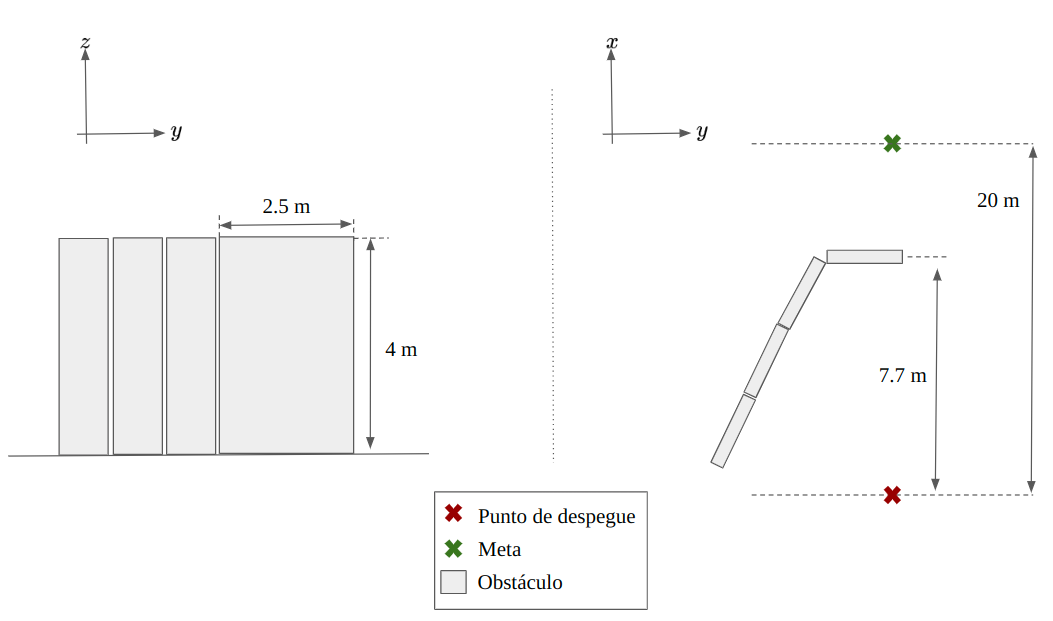
\includegraphics[scale=0.31]{partes/img/config-4-left-wall.png}
    \caption[Cuarta configuración de obstáculos dentro del entorno de AirSim.]{Cuarta configuración de obstáculos dentro del entorno de AirSim. Obstáculo simple con pared del lado izquierdo.}
    \label{fig:config-4-wall}
\end{figure}

Todos los vuelos realizados en esta configuración terminaron en una colisión. La Figura \ref{depth-wall-1}, la Figura \ref{depth-wall-2}, la Figura \ref{depth-wall-3}, la Figura \ref{depth-wall-4} y la Figura \ref{depth-wall-5} muestran una secuencia consecutiva de capturas de la visualización 3D de un vuelo en esta configuración que resultó en colisión. En las figuras se observa como la política de evasión de obstáculos intenta generar trayectorias que se dirigen hacia la región en la dirección \jim{-y_B} en donde no hay información de profundidad, probablemente esperando encontrar el borde del obstáculo en esa dirección, pero como en esta configuración de obstáculos ese borde se encuentra hacia atrás, se produce una colisión.

\begin{figure}[H]
    \centering
    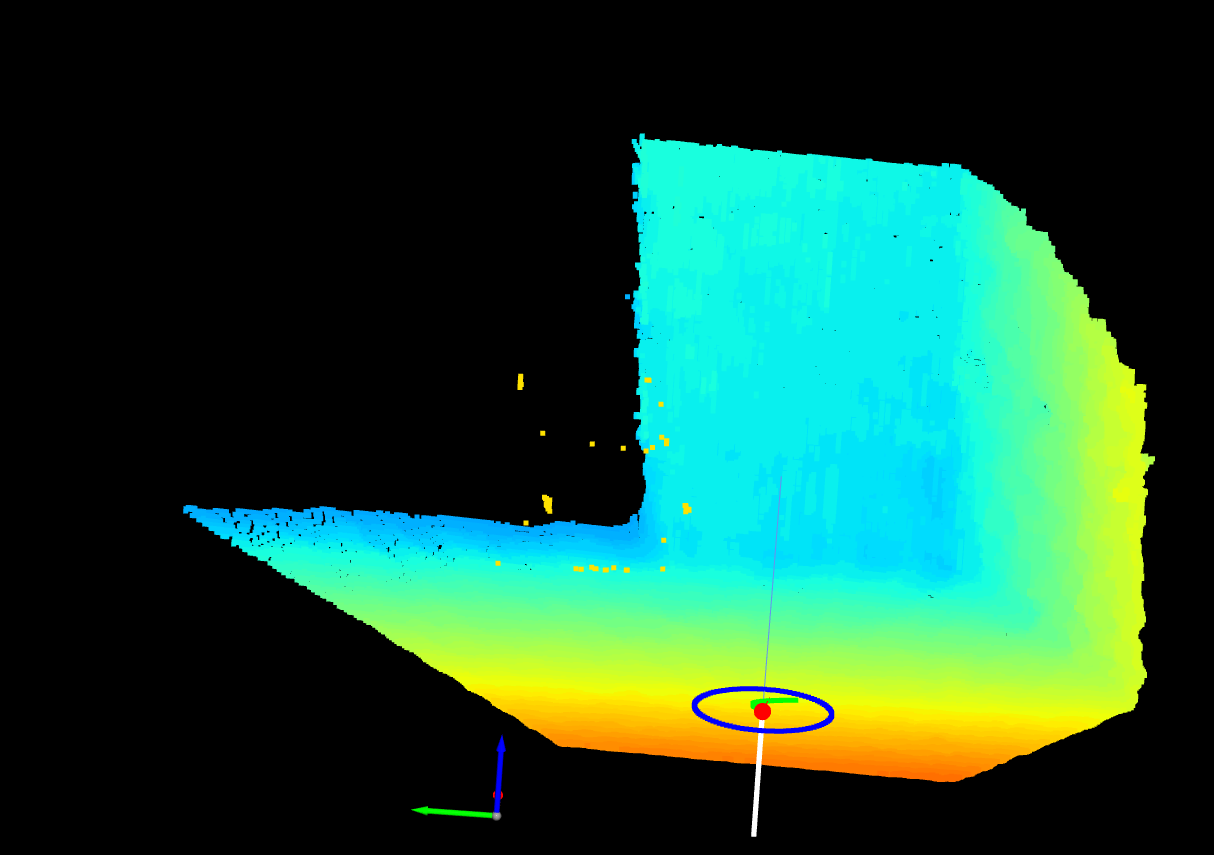
\includegraphics[scale=0.23]{partes/img/depth-wall-1-front.png}
    \caption[Visualización 3D de un vuelo en la cuarta configuración de obstáculos (1). Vista frontal.]{Visualización 3D de un vuelo en la cuarta configuración de obstáculos (1). Vista frontal.}
    \label{depth-wall-1}
\end{figure}

\begin{figure}[H]
    \centering
    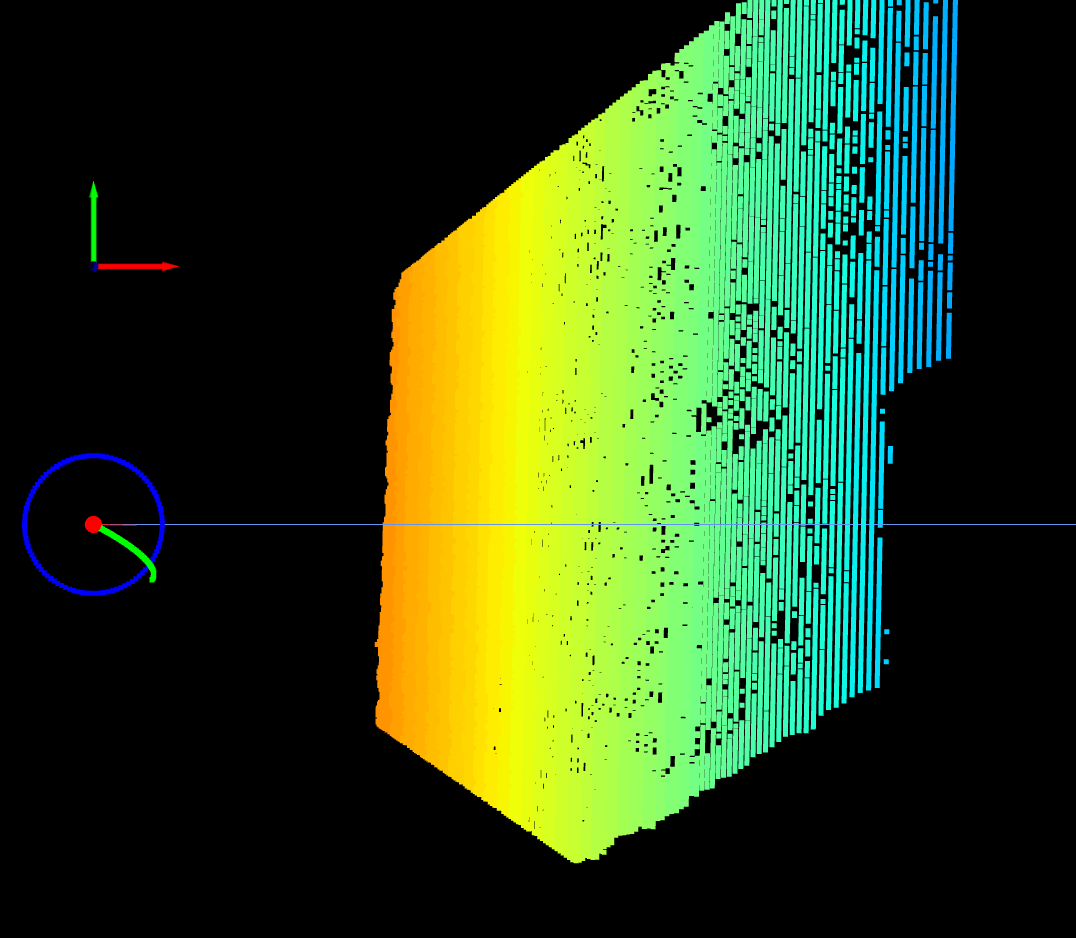
\includegraphics[scale=0.25]{partes/img/depth-wall-2-top.png}
    \caption[Visualización 3D de un vuelo en la cuarta configuración de obstáculos (2). Vista de arriba hacia abajo. Búsqueda del borde del obstáculo.]{Visualización 3D de un vuelo en la cuarta configuración de obstáculos (2). Vista de arriba hacia abajo. Las trayectorias se dirigen hacia la región en dirección \jim{-y_B} sin información de profundidad, probablemente buscando el borde del obstáculo.}
    \label{depth-wall-2}
\end{figure}

\begin{figure}[H]
    \centering
    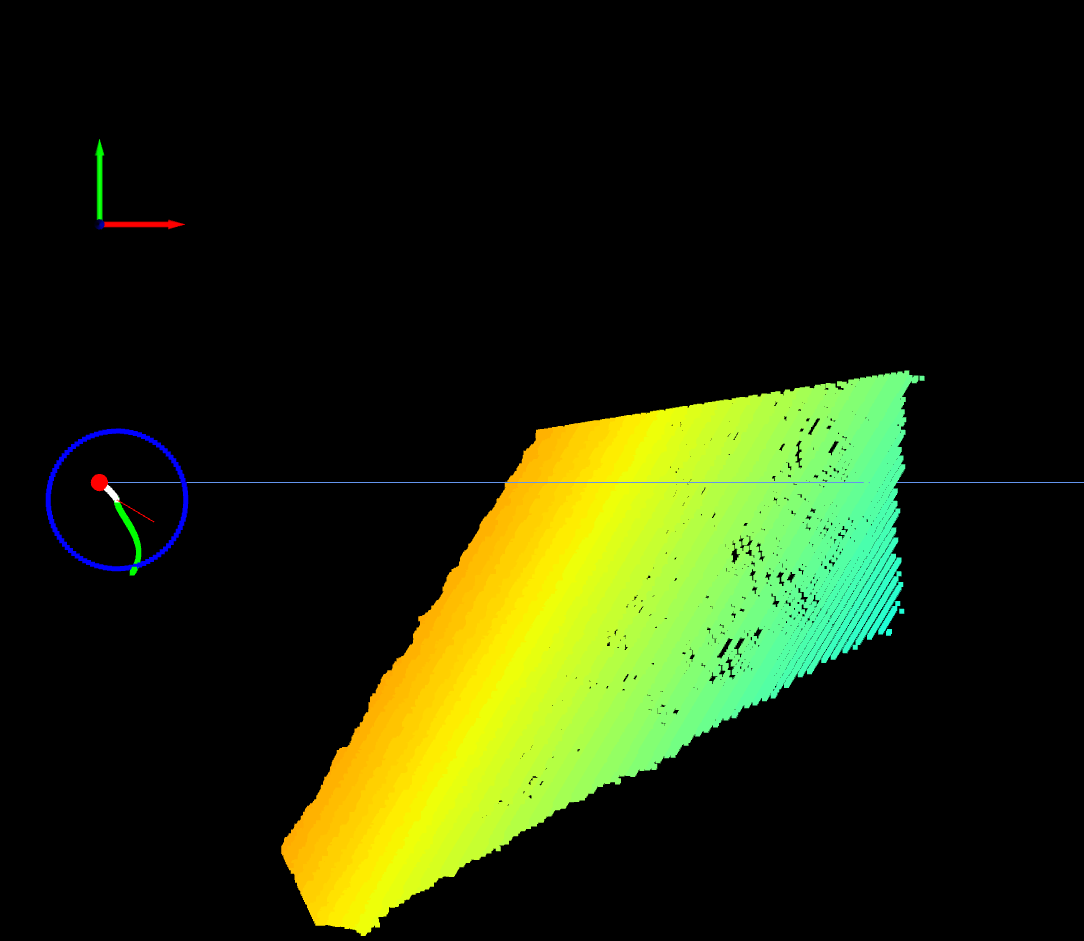
\includegraphics[scale=0.25]{partes/img/depth-wall-3-try-arround.png}
    \caption[Visualización 3D de un vuelo en la cuarta configuración de obstáculos (3). Vista de arriba hacia abajo. Búsqueda del borde del obstáculo.]{Visualización 3D de un vuelo en la cuarta configuración de obstáculos (3). Vista de arriba hacia abajo. Las trayectorias continúan dirigiéndose hacia la región en dirección \jim{-y_B} sin información de profundidad, probablemente buscando el borde del obstáculo.}
    \label{depth-wall-3}
\end{figure}

\begin{figure}[H]
    \centering
    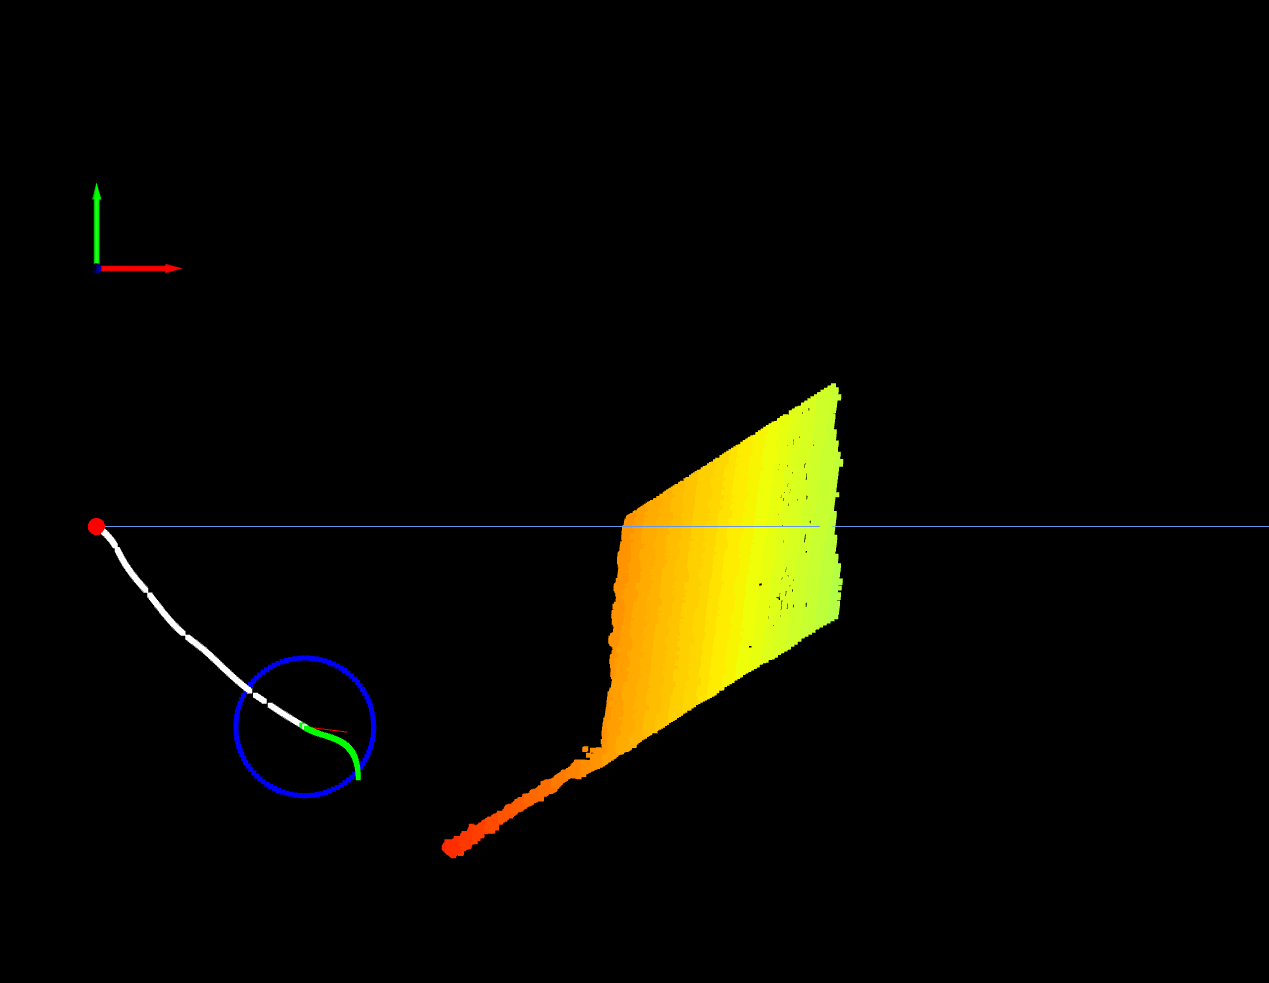
\includegraphics[scale=0.25]{partes/img/depth-wall-4-still-go-arround.png}
    \caption[Visualización 3D de un vuelo en la cuarta configuración de obstáculos (4). Vista de arriba hacia abajo. Búsqueda del borde del obstáculo.]{Visualización 3D de un vuelo en la cuarta configuración de obstáculos (4). Vista de arriba hacia abajo. Las trayectorias continúan dirigiéndose hacia la región en dirección \jim{-y_B} sin información de profundidad, probablemente buscando el borde del obstáculo.}
    \label{depth-wall-4}
\end{figure}

\begin{figure}[H]
    \centering
    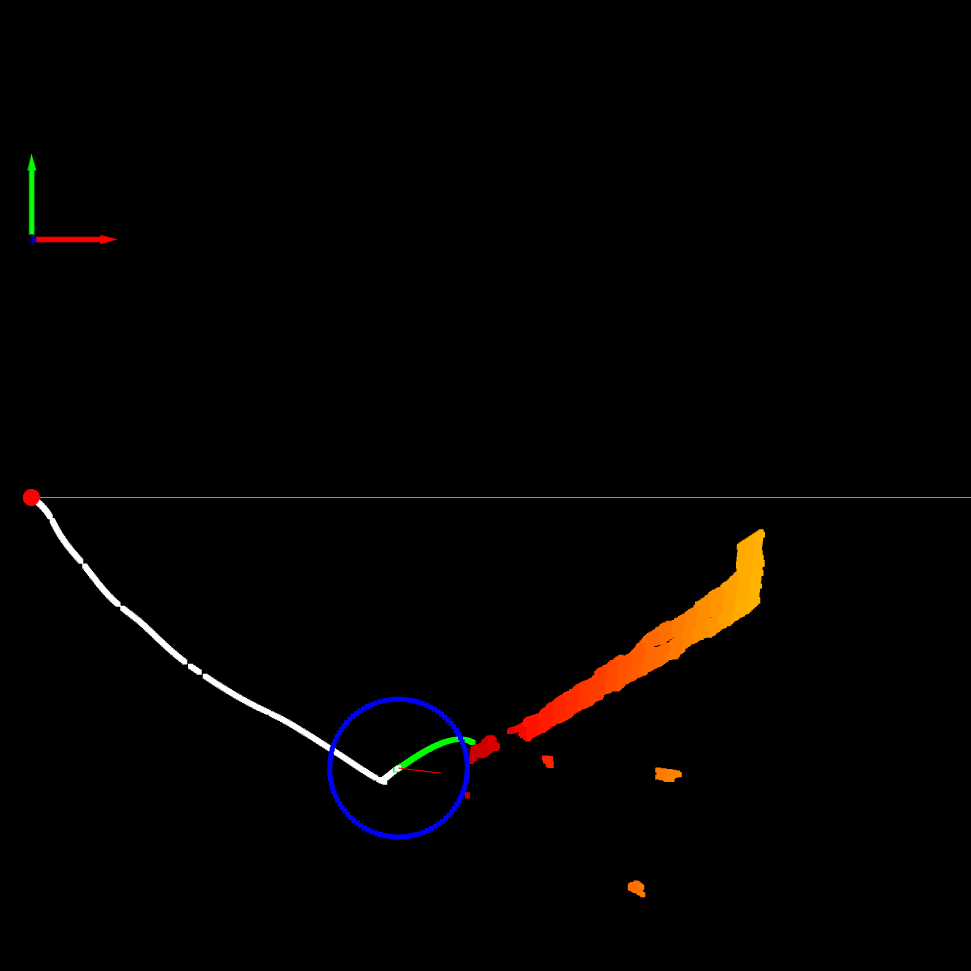
\includegraphics[scale=0.25]{partes/img/depth-wall-5-crash.png}
    \caption[Visualización 3D de un vuelo en la cuarta configuración de obstáculos (5). Vista de arriba hacia abajo. Colisión.]{Visualización 3D de un vuelo en la cuarta configuración de obstáculos. Vista de arriba hacia abajo. Al no conseguir el borde del obstáculo a tiempo, se produce una colisión.}
    \label{depth-wall-5}
\end{figure}

De estos resultados se confirma que los efectos consecuencia de las dificultades encontradas durante el refinamiento fino de la política estudiante son la preferencia certera a esquivar obstáculos hacia el flanco izquierdo (en dirección \jim{-y_B}), y que estos efectos producen colisiones en configuraciones de obstáculos donde no es posible esquivar hacia ese flanco.

En la Tabla \ref{table:sim-results} se muestra un resumen de los resultados obtenidos en los vuelos en simulación. En esta tabla se muestra que la política es estable para las configuraciones de obstáculos donde es trivial esquivar por el flanco izquierdo. De igual forma, se muestra que la política es inestable y propensa a producir colisiones para las configuraciones de obstáculos donde es no trivial esquivar por el flanco izquierdo.

\begin{table}[h]
\centering
\begin{tabular}{||c || c | c | c | c | c | c||} 
 \hline
 \textbf{Configuración} & \jim{N} & \jim{N_{e}} & \textbf{P} & \jim{\bar{D}} & \jim{\max(D)} & \jim{\min(D)} \rule{0pt}{2.6ex} \\ [0.4ex] 
 \hline\hline
 Obstáculo simple              & 10 & 10 & \textbf{100\%} & 3.1 & 3.4 & 2.7 \\ 
 \hline
 Dos obstáculos consecutivos   & 10 & 10 & \textbf{100\%} & 3.7 & 4 & 3.3 \\
 \hline
 Dos obstáculos paralelos      & 10 & 2  & \textbf{20 \%} & N/A & N/A & N/A \\
 \hline
 Obstáculo con pared izquierda & 10 & 0  & \textbf{0  \%} & N/A & N/A & N/A \\
 \hline
\end{tabular}
\caption[Resumen de los resultados obtenidos en los vuelos en simulación.]{Resumen de los resultados obtenidos en los vuelos en simulación. \jim{N} y \jim{N_{e}} son el número de vuelos totales y sin colisión respectivamente. \textbf{P} es el porcentaje de vuelos sin colisión. \jim{\bar{D}}, \jim{\max(D)} y \jim{\min(D)} son la desviación máxima promedio, máxima y mínima respectivamente (en metros).}
\label{table:sim-results}
\end{table}

\subsection{Vuelos sobre la plataforma física}

\label{sec:results-SOTEN}

En esta sección se describen las configuraciones y resultados de los vuelos realizados sobre la plataforma física de implementación (QUAV SOTEN\footnote[1]{En la Figura \ref{fig:SOTEN} se muestra al QUAV SOTEN.}) en un entorno de la vida real. Esto vuelos fueron ejecutados en un campo de vuelo para drones ubicado en la prefectura de Chiba, Japón; las condiciones climáticas del día fueron: soleado con un ligero viento en dirección hacia el oeste. Durante los vuelos, un piloto experto estuvo preparado para controlar manualmente el QUAV en caso de que una colisión fuera inminente. En esta sección se utiliza el termino ``colision'' para referirse al evento de interrumpir el vuelo autónomo para evitar una colisión inminente. Al igual que durante los vuelos en simulación, la ejecución de la evasión de obstáculos está limitada al plano \jim{xy} del marco de referencia del cuerpo del QUAV.

La primera configuración de obstáculos utilizada fue una configuración simple con un solo obstáculo en la línea directa de visión del QUAV, la Figura \ref{real-1-single-0-setup} muestra una fotografía ilustrada que describe la configuración.

\begin{figure}[H]
    \centering
    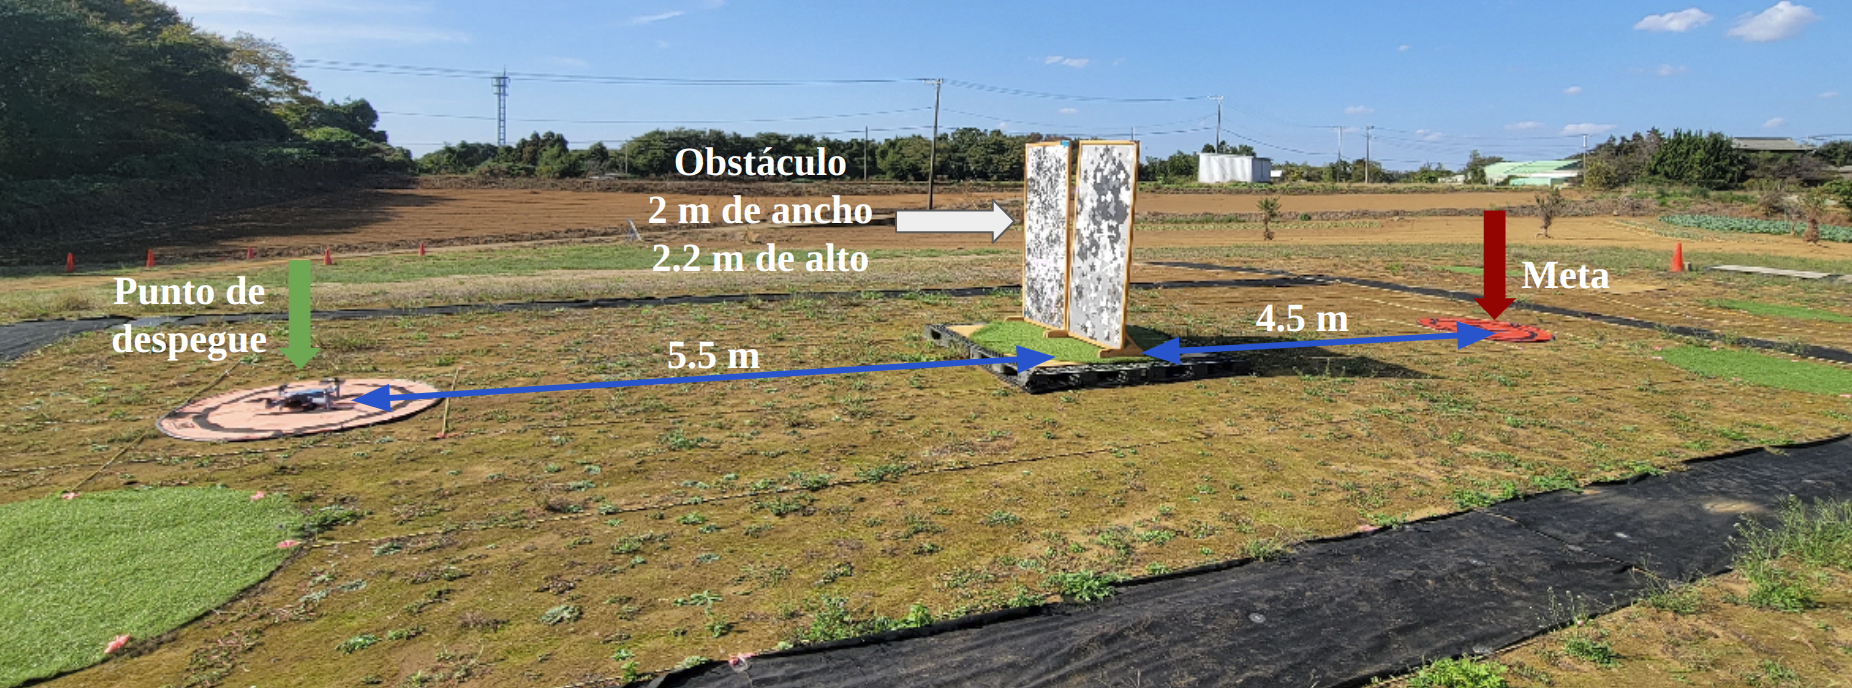
\includegraphics[scale=0.22]{partes/img/real-1-single-0-setup.png}
    \caption[Configuración de obstáculos en entorno real: Obstáculo simple]{Configuración de obstáculos en entorno real: Obstáculo simple.}
    \label{real-1-single-0-setup}
\end{figure}

Se realizaron 11 vuelos en esta configuración, y los resultados fueron análogos a los obtenidos en simulación, en concreto, de 11 vuelos ejecutados, 10 resultaron sin colisión y uno fue abortado por el piloto debido a la influencia de una fuerte ráfaga de viento. Los caminos resultantes de los vuelos también fueron análogos a los obtenidos en simulación, sin embargo, debido a variaciones en el viento y en las condiciones de iluminación, algunas ejecuciones se desviaron considerablemente del camino directo. La Figura \ref{real-1-single-graph} muestra una visualización de arriba hacia abajo de 10 de los caminos ejecutados en esta configuración, incluyendo el vuelo que fue abortado por el piloto. Se puede observar que la desviación máxima de los caminos ejecutados con respecto al camino directo entre el punto de despegue y la meta varía bastante entre vuelos (probablemente debido a las variaciones en el viento), la Figura \ref{real-1-single-box} muestra un diagrama de caja de la desviación máxima de los caminos ejecutados en esta configuración. La desviación máxima promedio de los caminos ejecutados en esta configuración es cerca de 3.2 metros, con una desviación máxima de cerca de 4.5 metros y una desviación mínima de cerca de 2 metros.

\begin{figure}[H]
    \centering
    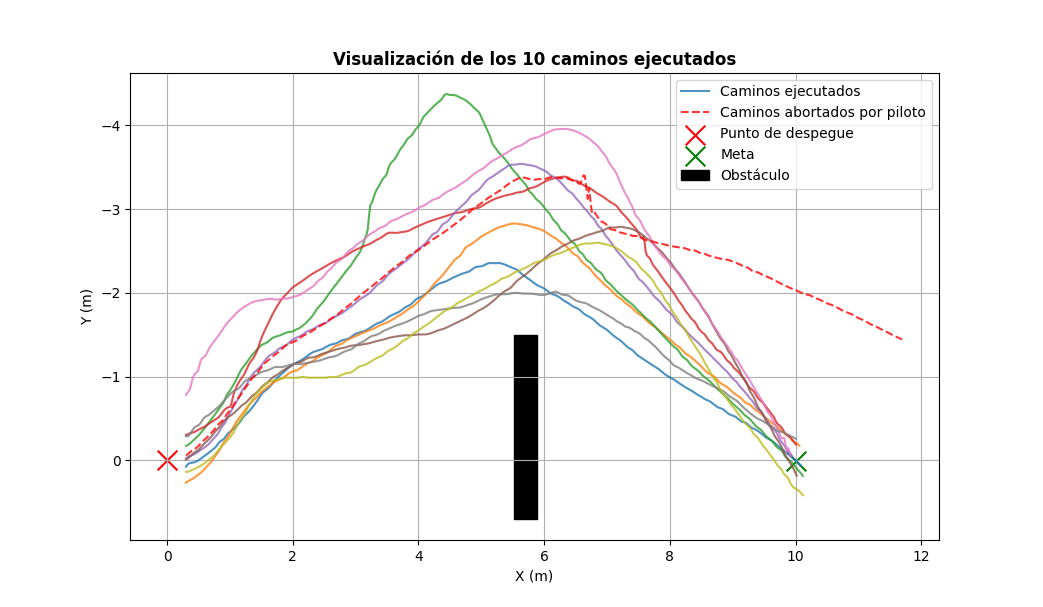
\includegraphics[scale=0.55]{partes/img/real-1-single-graph-all.png}
    \caption[Visualización de 10 caminos ejecutados en la primera configuración de obstáculos en entorno real.]{Visualización de 10 caminos ejecutados en la primera configuración de obstáculos en entorno real. Incluyendo el vuelo que fue abortado por el piloto.}
    \label{real-1-single-graph}
\end{figure}

\begin{figure}[H]
    \centering
    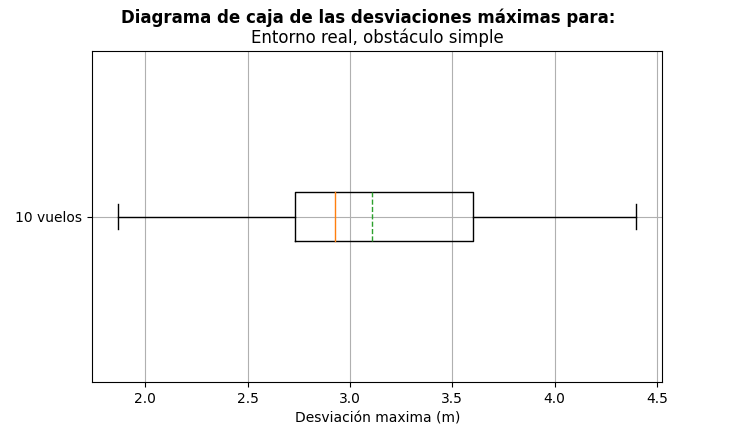
\includegraphics[scale=0.7]{partes/img/real-1-single-box.png}
    \caption[Diagrama de caja de la desviación máxima de los caminos ejecutados en la primera configuración de obstáculos en entorno real.]{Diagrama de caja de la desviación máxima de los caminos ejecutados en la primera configuración de obstáculos en entorno real.}
    \label{real-1-single-box}
\end{figure}

En todos los vuelos ejecutados en esta configuración, el algoritmo esquivó el obstáculo por el flanco izquierdo y continuo en dirección a la meta. La Figura \ref{real-1-single-3-frames-1}, la Figura \ref{real-1-single-3-frames-2} y la Figura \ref{real-1-single-3-frames-3} muestran capturas de una grabación de uno de los vuelos sobre esta configuración. La Figura \ref{real-1-single-4-frames-1}, la Figura \ref{real-1-single-4-frames-2} y la Figura \ref{real-1-single-4-frames-3} también muestran capturas de una grabación de uno de los vuelos sobre esta configuración pero en una perspectiva diferente. En estas figuras se aprecia claramente el comportamiento del algoritmo, en particular: comenzar el vuelo, esquivar el obstáculo por el flanco izquierdo, continuar avanzando hasta que se termine la trayectoria actual y finalmente, como no se observan obstáculos, navegar en dirección a la meta.

\begin{figure}[H]
    \centering
    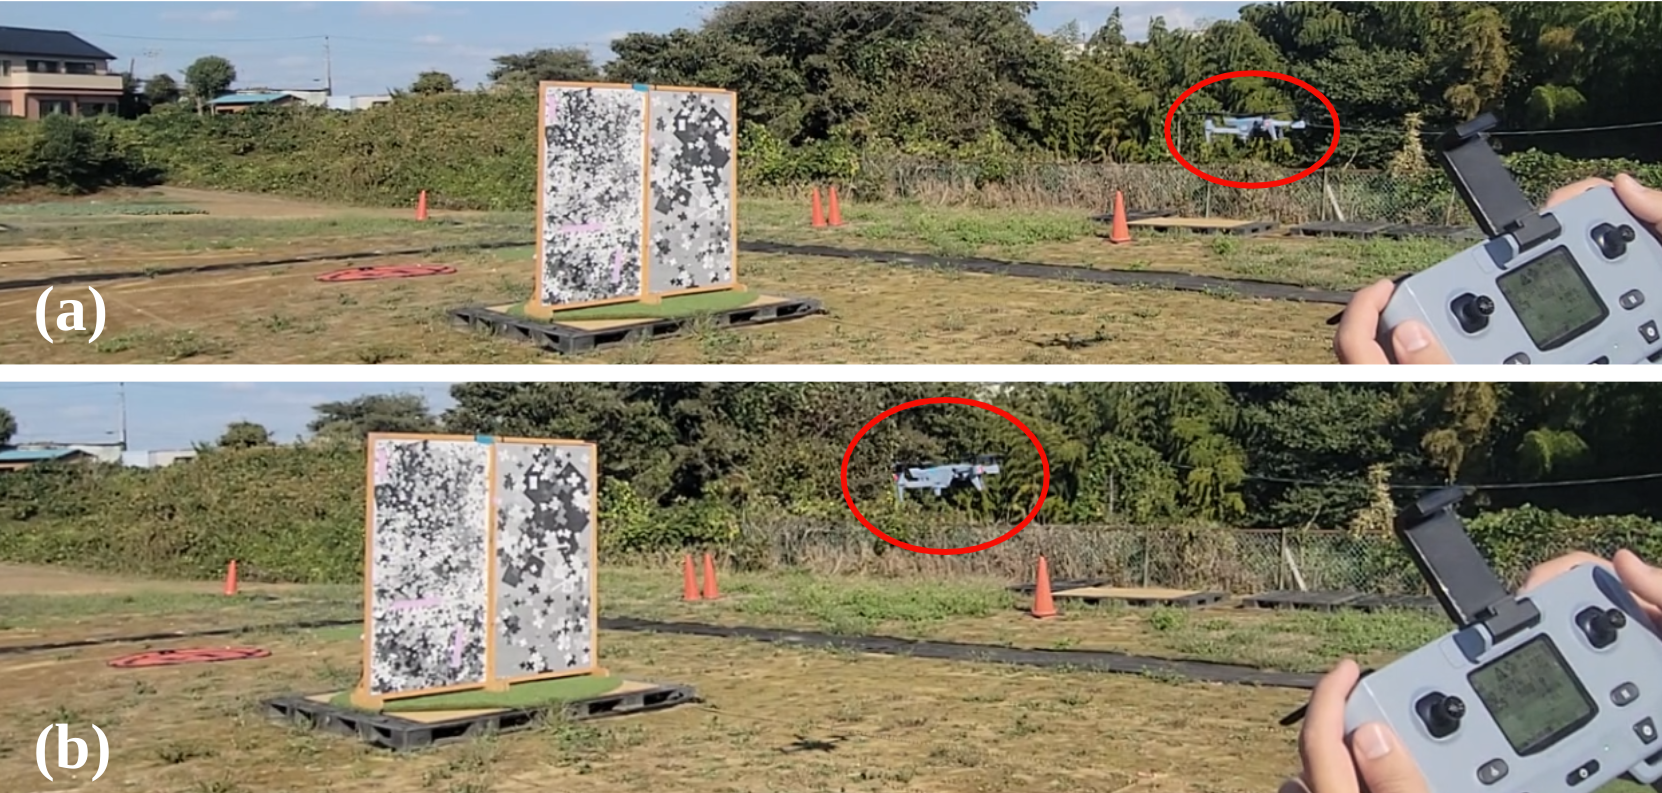
\includegraphics[scale=0.25]{partes/img/real-1-single-3-frames-1.png}
    \caption[Capturas de una grabación de uno de los vuelos en entorno real con un obstáculo simple (1).]{Capturas de una grabación de uno de los vuelos en entorno real con un obstáculo simple (1). \textbf{(a)} Comienza el vuelo. \textbf{(b)} Se comienza a esquivar el obstáculo.}
    \label{real-1-single-3-frames-1}
\end{figure}

\begin{figure}[H]
    \centering
    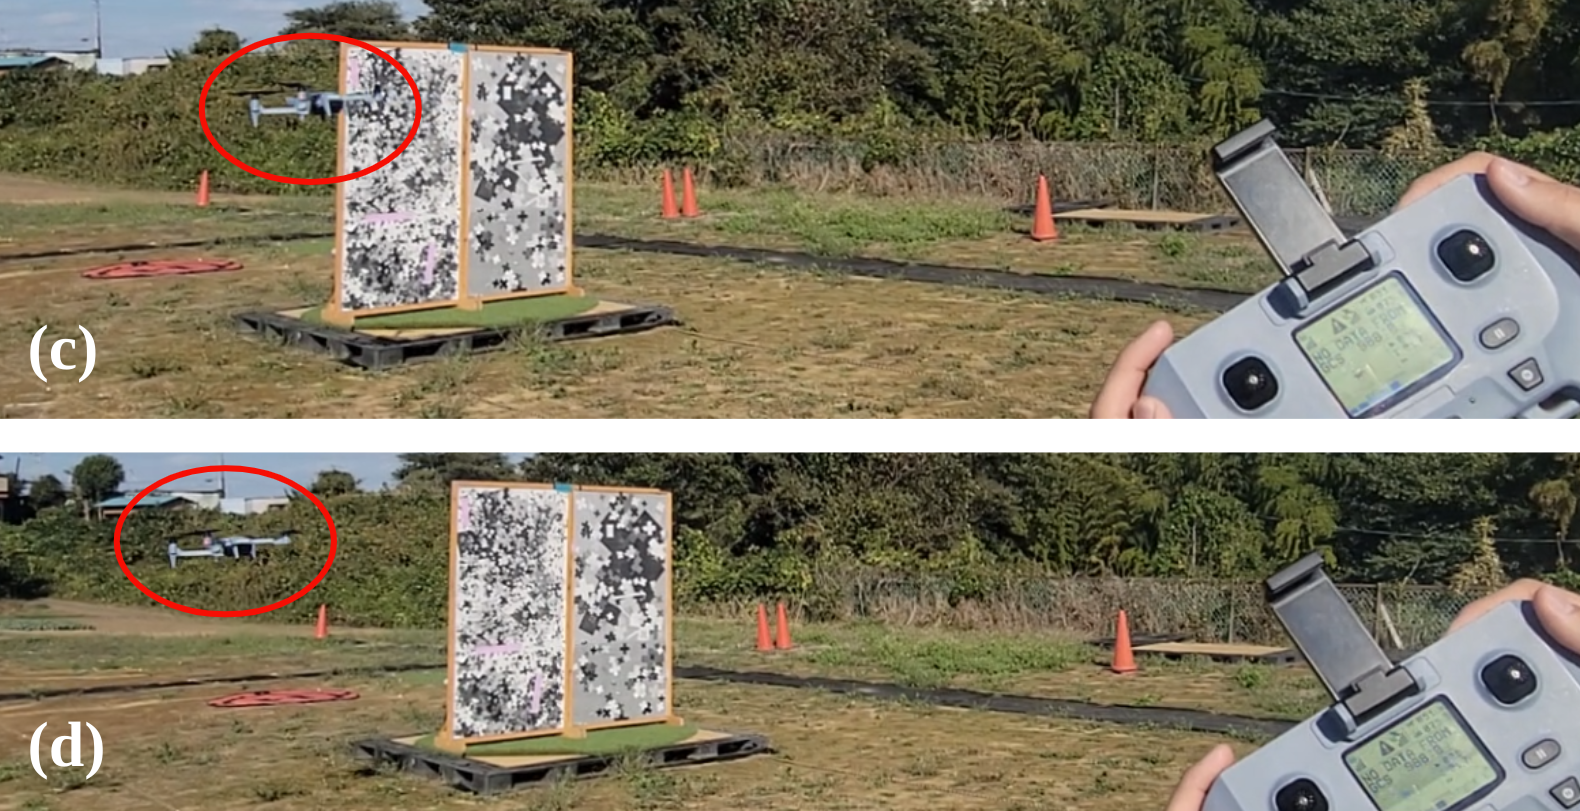
\includegraphics[scale=0.255]{partes/img/real-1-single-3-frames-2.png}
    \caption[Capturas de una grabación de uno de los vuelos en entorno real con un obstáculo simple (2).]{Capturas de una grabación de uno de los vuelos en entorno real con un obstáculo simple (2). En \textbf{(c)} y \textbf{(d)}, se esquiva el obstáculo por el flanco izquierdo.}
    \label{real-1-single-3-frames-2}
\end{figure}

\begin{figure}[H]
    \centering
    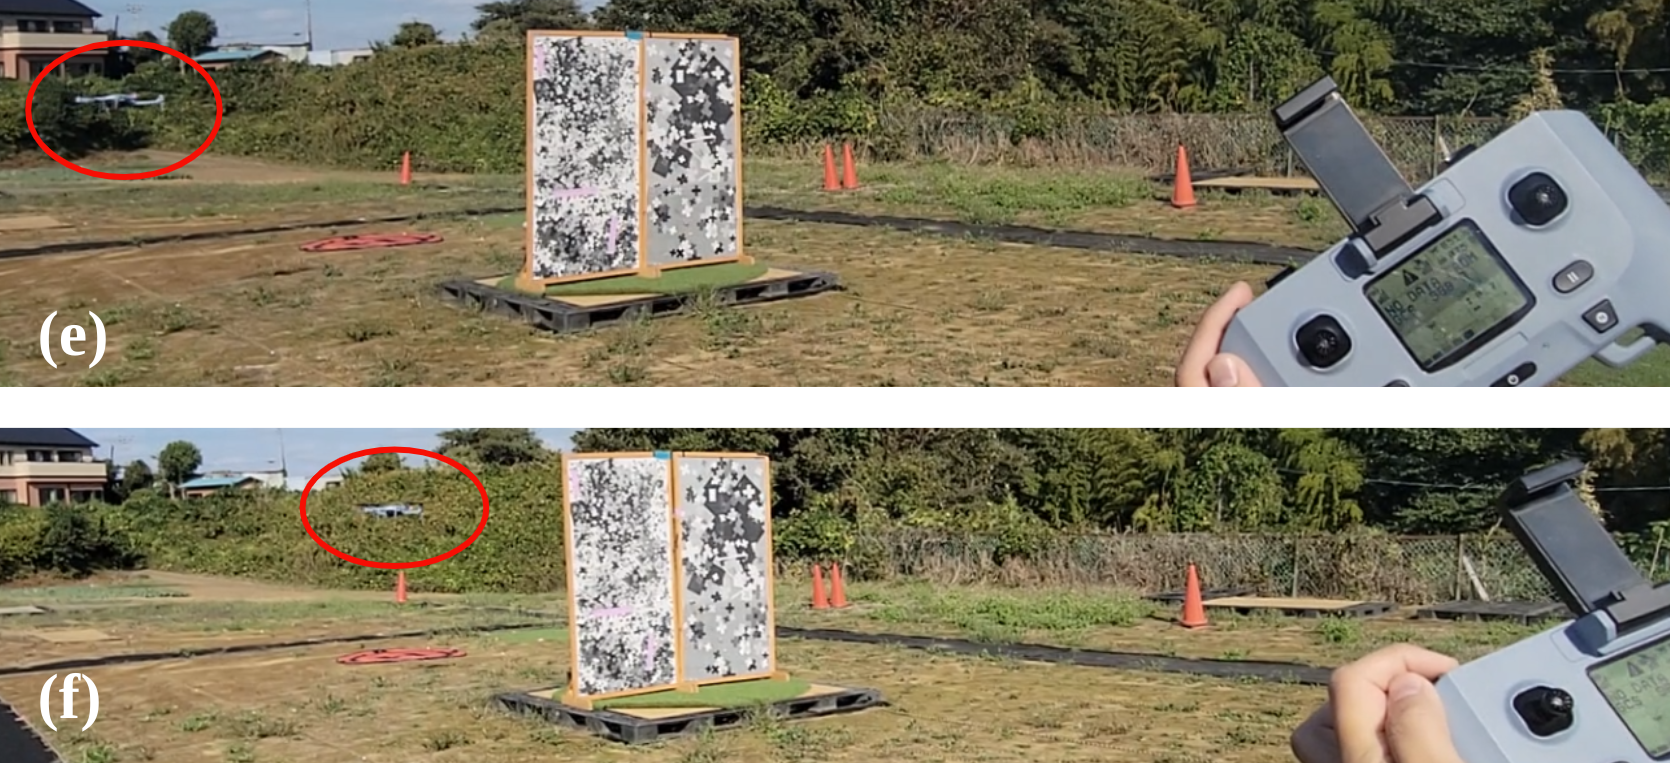
\includegraphics[scale=0.245]{partes/img/real-1-single-3-frames-3.png}
    \caption[Capturas de una grabación de uno de los vuelos en entorno real con un obstáculo simple (3).]{Capturas de una grabación de uno de los vuelos en entorno real con un obstáculo simple (3). En \textbf{(e)} y \textbf{(f)}, como no se observan obstáculos, se navega en dirección a la meta.}
    \label{real-1-single-3-frames-3}
\end{figure}

\begin{figure}[H]
    \centering
    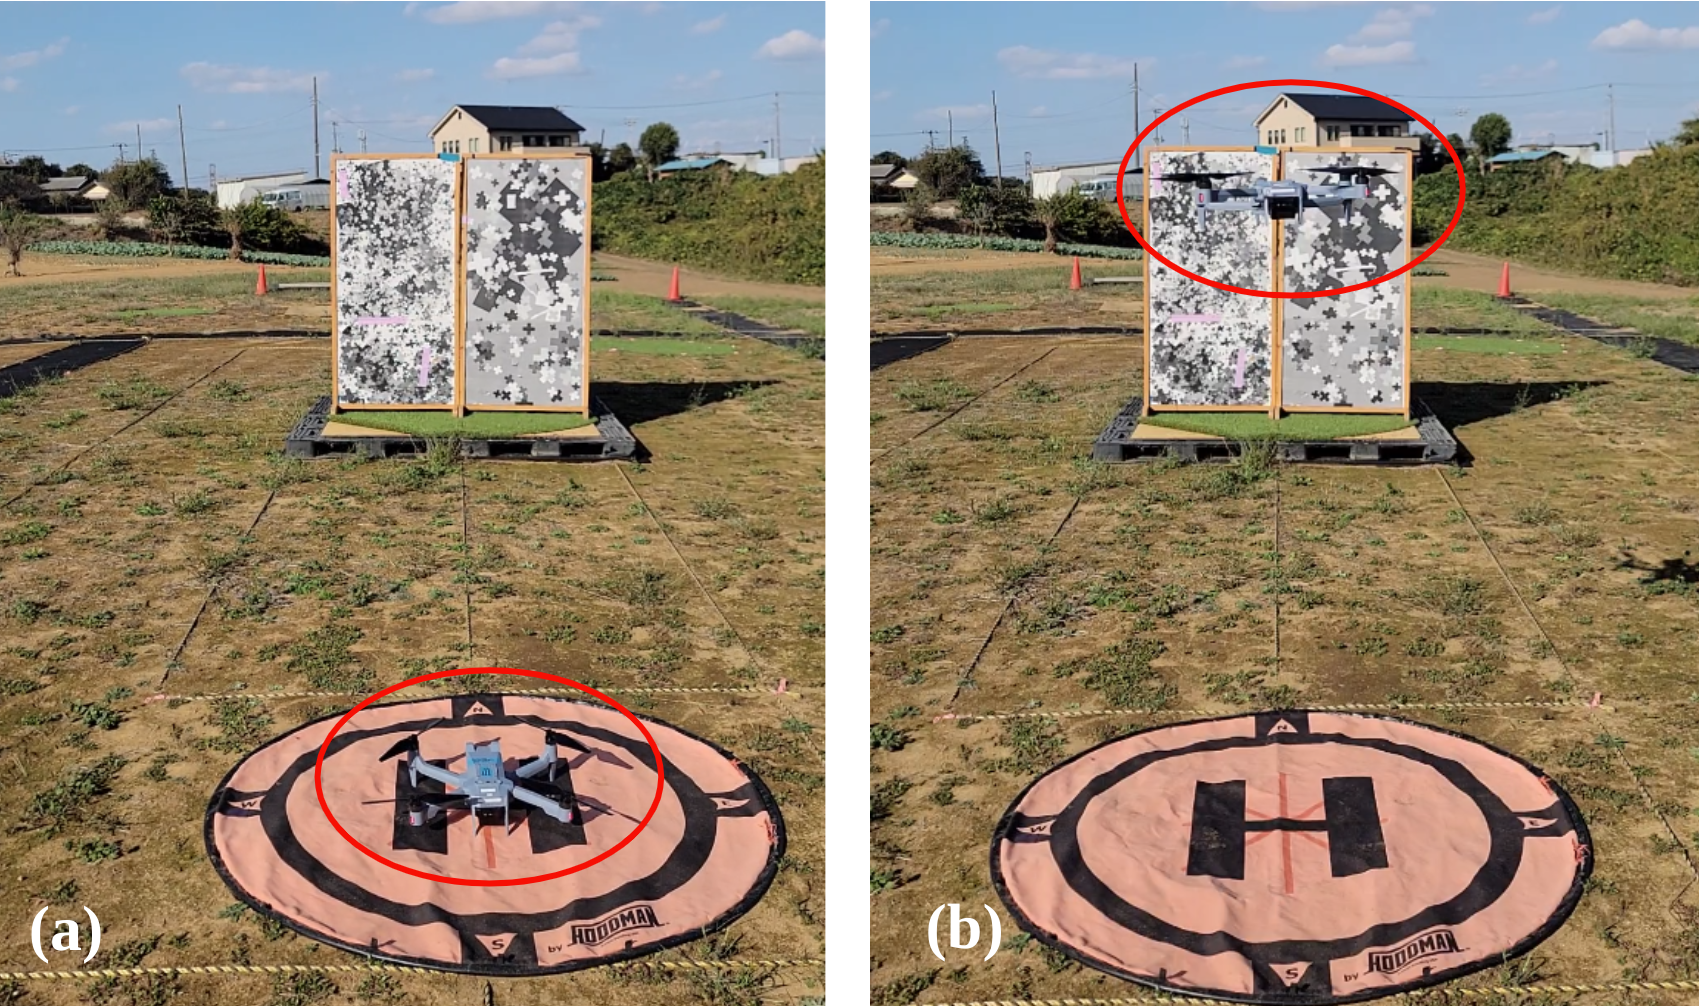
\includegraphics[scale=0.24]{partes/img/real-1-single-4-frames-1.png}
    \caption[Capturas de una grabación de uno de los vuelos en entorno real con un obstáculo simple. Vista frontal (1).]{Capturas de una grabación de uno de los vuelos en entorno real con un obstáculo simple. Vista frontal (1). \textbf{(a)} Antes del despegue. \textbf{(b)} Comienza el vuelo.}
    \label{real-1-single-4-frames-1}
\end{figure}

\begin{figure}[H]
    \centering
    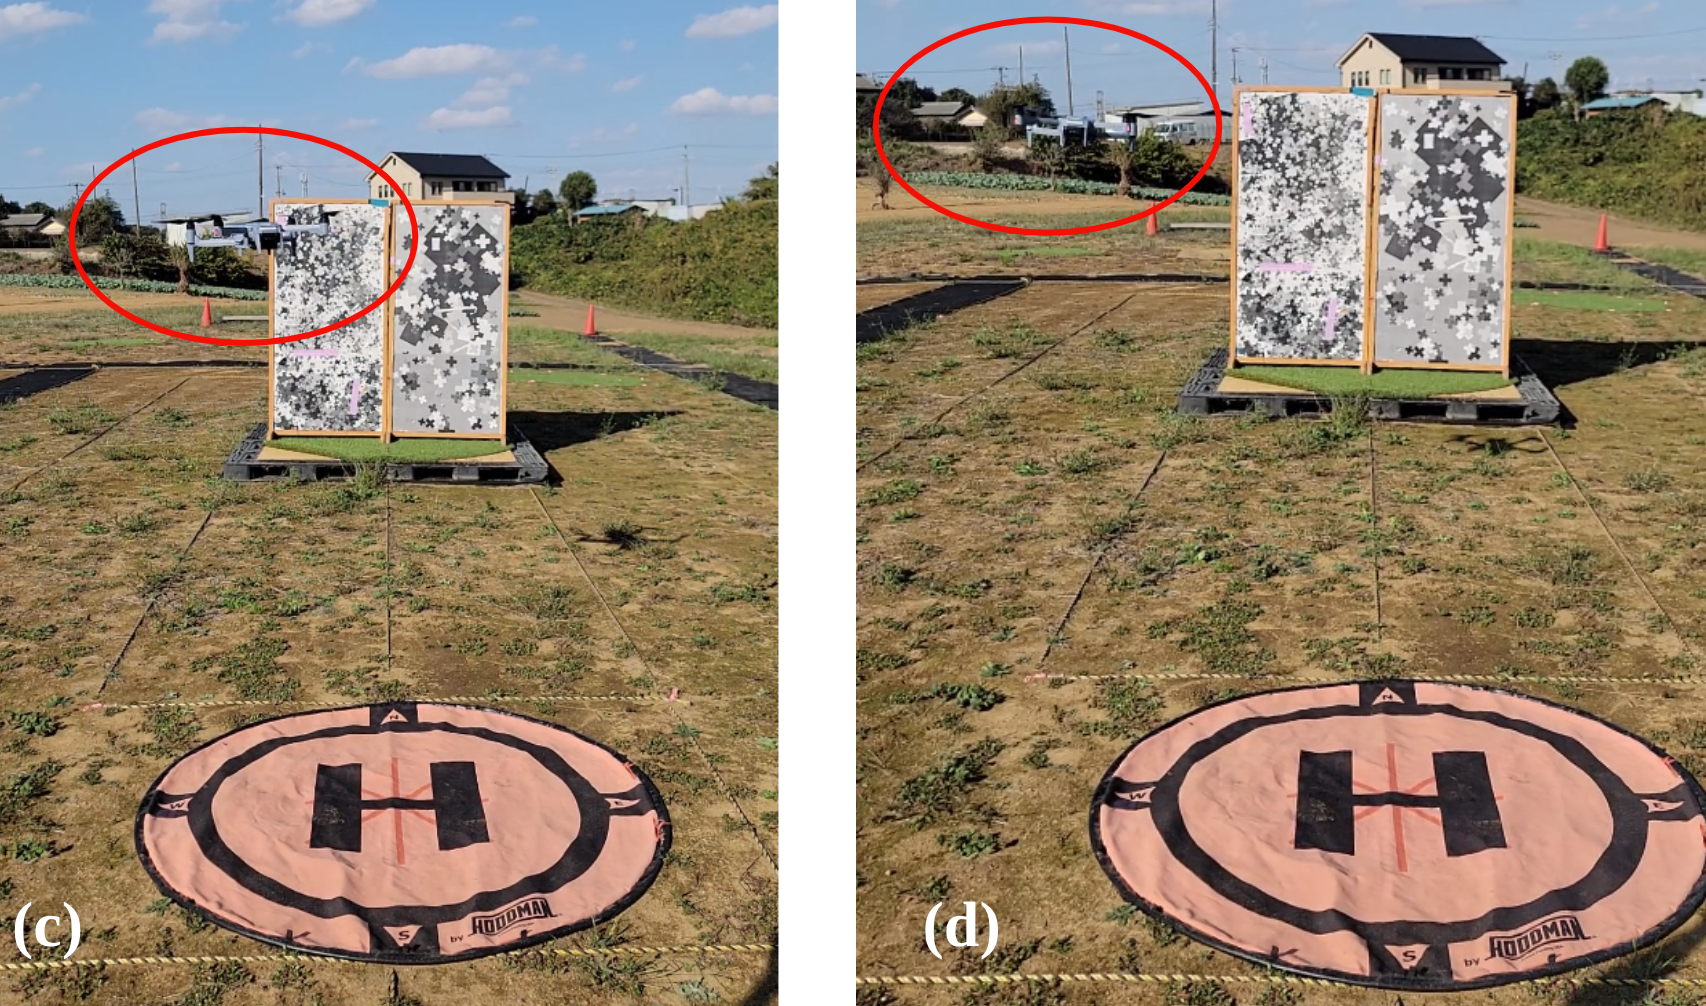
\includegraphics[scale=0.24]{partes/img/real-1-single-4-frames-2.png}
    \caption[Capturas de una grabación de uno de los vuelos en entorno real con un obstáculo simple. Vista frontal (2).]{Capturas de una grabación de uno de los vuelos en entorno real con un obstáculo simple. Vista frontal (2). En \textbf{(c)} y \textbf{(d)}, se esquiva el obstáculo por el flanco izquierdo.}
    \label{real-1-single-4-frames-2}
\end{figure}

\begin{figure}[H]
    \centering
    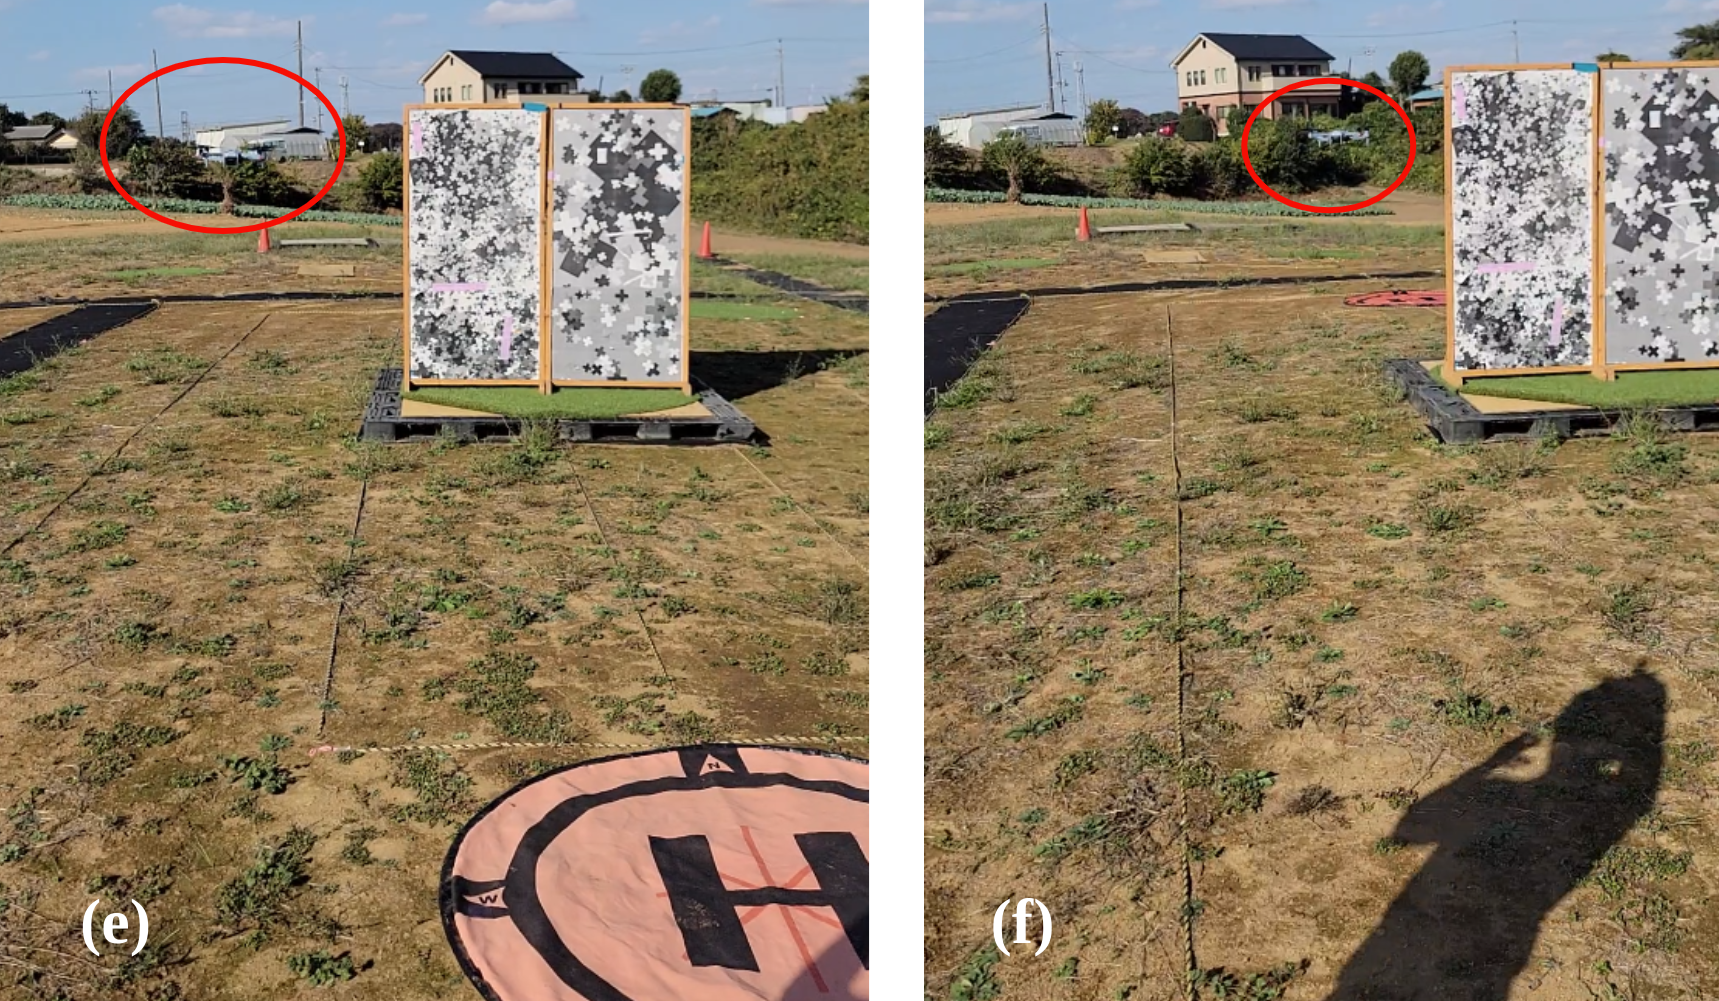
\includegraphics[scale=0.24]{partes/img/real-1-single-4-frames-3.png}
    \caption[Capturas de una grabación de uno de los vuelos en entorno real con un obstáculo simple. Vista frontal (3).]{Capturas de una grabación de uno de los vuelos en entorno real con un obstáculo simple. Vista frontal (3). En \textbf{(e)} y \textbf{(f)}, como no se observan obstáculos, se navega en dirección a la meta.}
    \label{real-1-single-4-frames-3}
\end{figure}

La segunda configuración de obstáculos utilizada fue una configuración con dos obstáculos paralelos con una separación entre si, esta separación fue distinta para cada vuelo. A diferencia de la configuración anterior, en esta configuración solo se hicieron 3 vuelos. El objetivo de estos vuelos era observar el comportamiento del algoritmo en este escenario, en particular, confirmar la presencia de la tendencia certera de esquivar obstáculos por el flanco izquierdo que se observó durante vuelos análogos en entornos de simulación; así como también observar si esta tendencia produce colisiones inminentes.

En el primer vuelo en esta configuración se utilizó una separación de 3 metros, la Figura \ref{real-2-parallelA-0-config} muestra una fotografía que ilustra la configuración utilizada. Este vuelo fue abortado por colisión inminente, la Figura \ref{real-2-parallelA-1-frames} muestra capturas de la grabación de este vuelo en donde se observa el comportamiento del algoritmo. Primero (Figura \ref{real-2-parallelA-1-frames}(a)), la ejecución comienza; segundo (Figura \ref{real-2-parallelA-1-frames}(b)), el QUAV se dirige hacia el espacio entre ambos obstáculos en lugar de esquivar los obstáculos por el flanco derecho; y tercero (Figura \ref{real-2-parallelA-1-frames}(c)), cuando el obstáculo derecho sale del campo de visión, el algoritmo intenta esquivar el obstáculo que aun es visible por el flanco izquierdo, lo cual produce una colisión inminente, haciendo que el piloto tenga que abortar el vuelo. Estos resultados coinciden con el comportamiento observado en simulación \footnote[1]{Vea la Figura \ref{fig:depth-parallel-5}}, y confirman la presencia de la tendencia certera a esquivar obstáculos por el flanco izquierdo.

\begin{figure}[H]
    \centering
    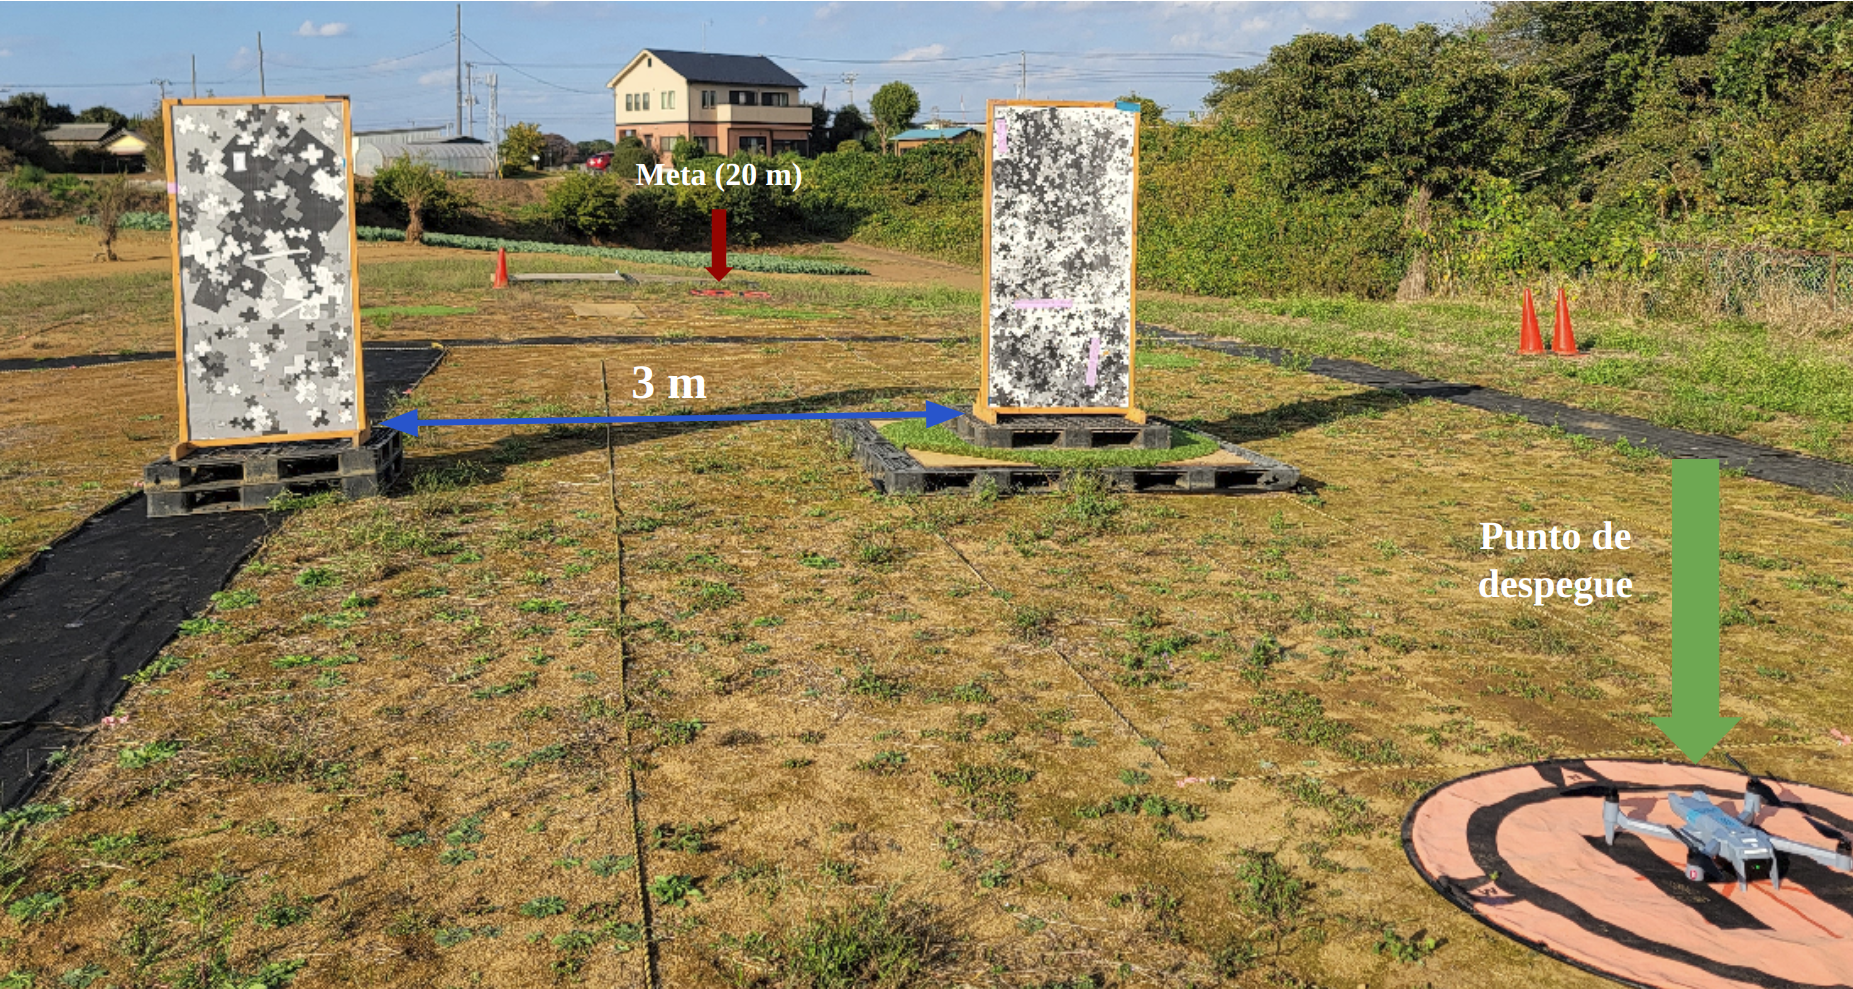
\includegraphics[scale=0.22]{partes/img/real-2-parallelA-0-config.png}
    \caption[Configuración de obstáculos en entorno real: Obstáculos paralelos a 3 metros de separación.]{Configuración de obstáculos en entorno real: Obstáculos paralelos a 3 metros de separación.}
    \label{real-2-parallelA-0-config}
\end{figure}

\begin{figure}[H]
    \centering
    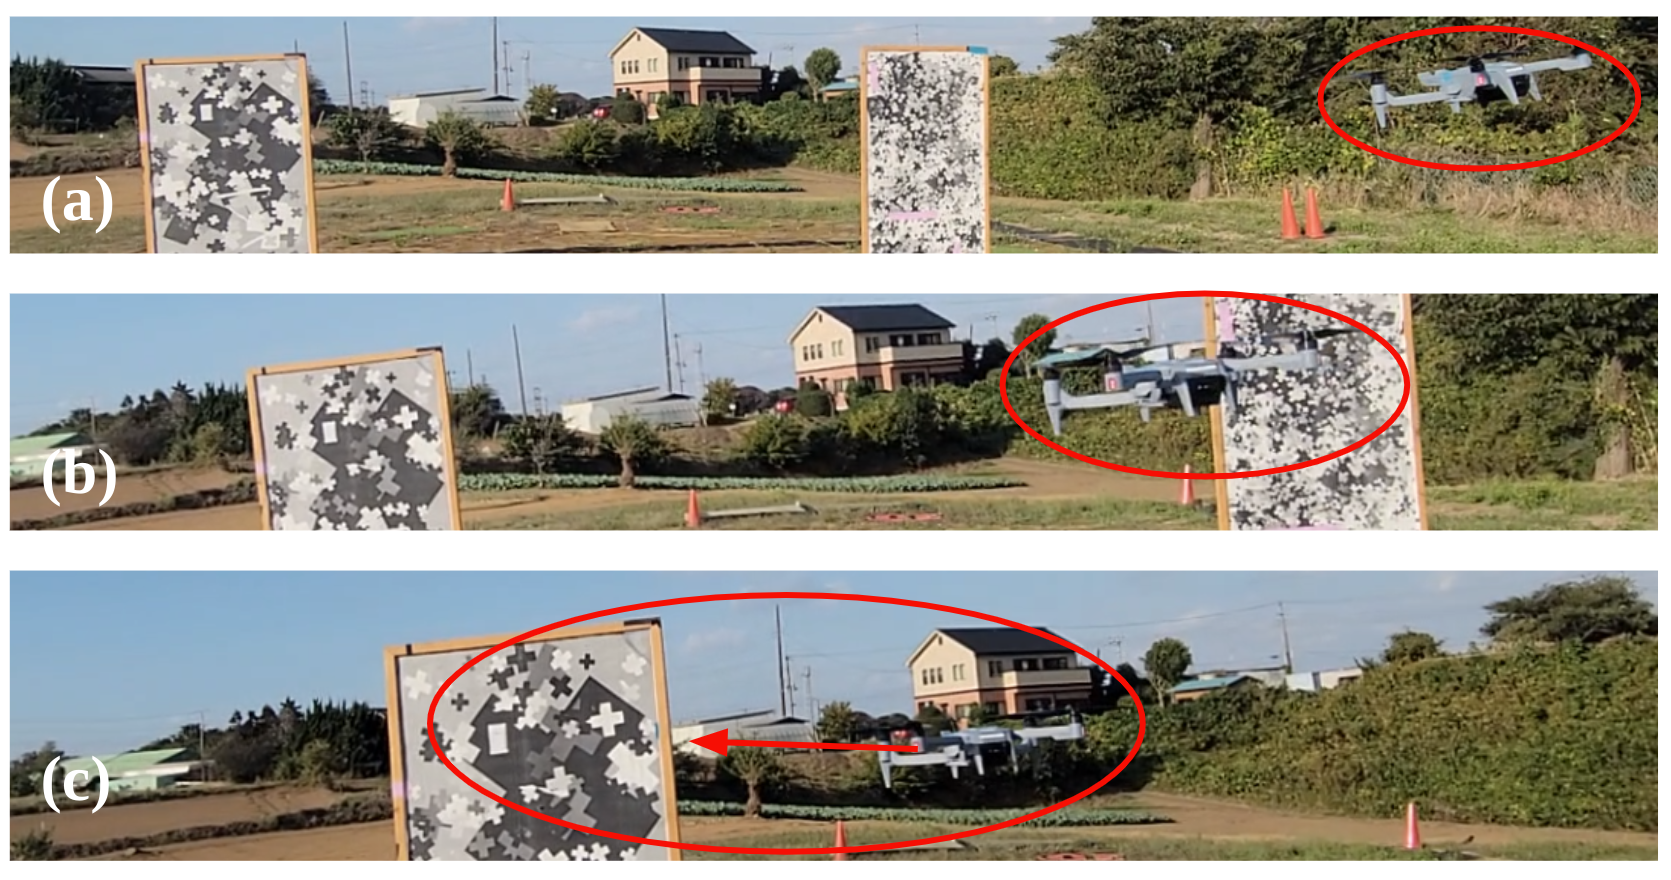
\includegraphics[scale=0.25]{partes/img/real-2-parallelA-1-frames.png}
    \caption[Capturas de la grabación del vuelo en entorno real con obstáculos paralelos a 3 metros de separación.]{Capturas de la grabación del vuelo en entorno real con obstáculos paralelos a 3 metros de separación. \textbf{(a)} La ejecución comienza. \textbf{(b)} El QUAV se dirige hacia el espacio entre ambos obstáculos en lugar de esquivar los obstáculos por el flanco derecho. \textbf{(c)} Cuando el obstáculo derecho sale del campo de visión, el algoritmo intenta esquivar el obstáculo que aun es visible por el flanco izquierdo, lo cual produce una colisión inminente.}
    \label{real-2-parallelA-1-frames}
\end{figure}

El segundo vuelo en la configuración de obstáculos paralelos utilizó una separación de 4 metros, la Figura \ref{real-3-parallelB-0-config} muestra una fotografía que ilustra la configuración utilizada. Este vuelo resultó exitoso, la Figura \ref{real-3-parallelB-1-frames} muestra capturas de la grabación de este vuelo en donde se observa el comportamiento del algoritmo. Primero (Figura \ref{real-3-parallelB-1-frames}(a)), la ejecución comienza y el QUAV navega hacia el espacio entre los dos obstáculos; segundo (Figura \ref{real-3-parallelB-1-frames}(b)), esta vez, el obstáculo izquierdo sale del campo de visión, y el QUAV continúa hacia el espacio entre los dos obstáculos; y tercero (Figura \ref{real-3-parallelB-1-frames}(c)), se superan los obstáculos y se navega en dirección a la meta. De este vuelo confirmamos que si la configuración de obstáculos paralelos es tal que el primer obstáculo que desaparece el campo de visión es el obstáculo izquierdo, entonces es posible que el algoritmo sea capaz de completar el vuelo sin producir colisiones. La Figura \ref{real-3-parallelB-2-graph} muestra una visualización de arriba hacia abajo del camino ejecutado por el QUAV en este vuelo.

\begin{figure}[H]
    \centering
    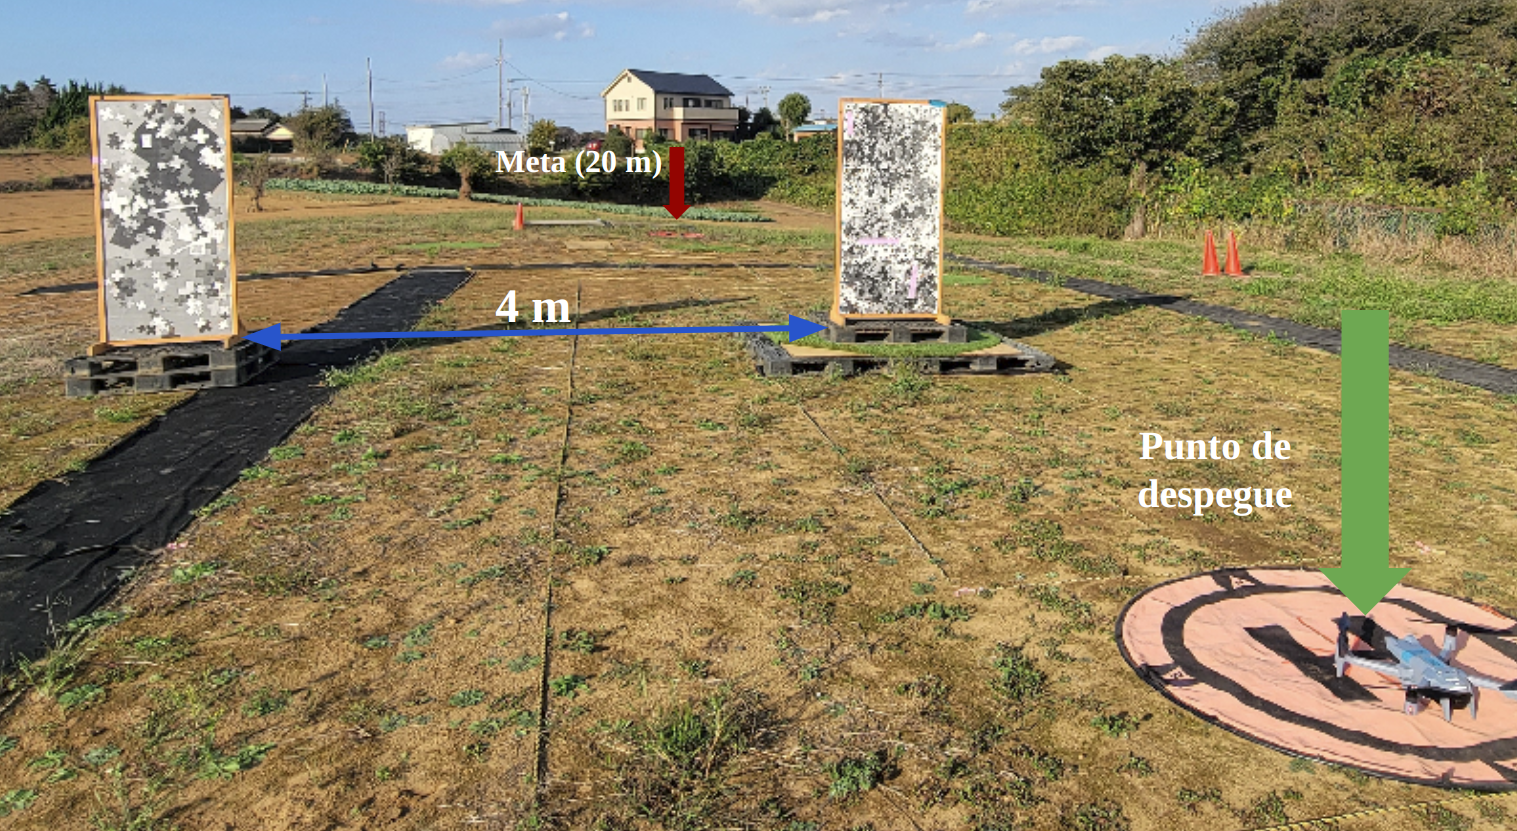
\includegraphics[scale=0.27]{partes/img/real-3-parallelB-0-config.png}
    \caption[Configuración de obstáculos en entorno real: Obstáculos paralelos a 4 metros de separación.]{Configuración de obstáculos en entorno real: Obstáculos paralelos a 4 metros de separación.}
    \label{real-3-parallelB-0-config}
\end{figure}

\begin{figure}[H]
    \centering
    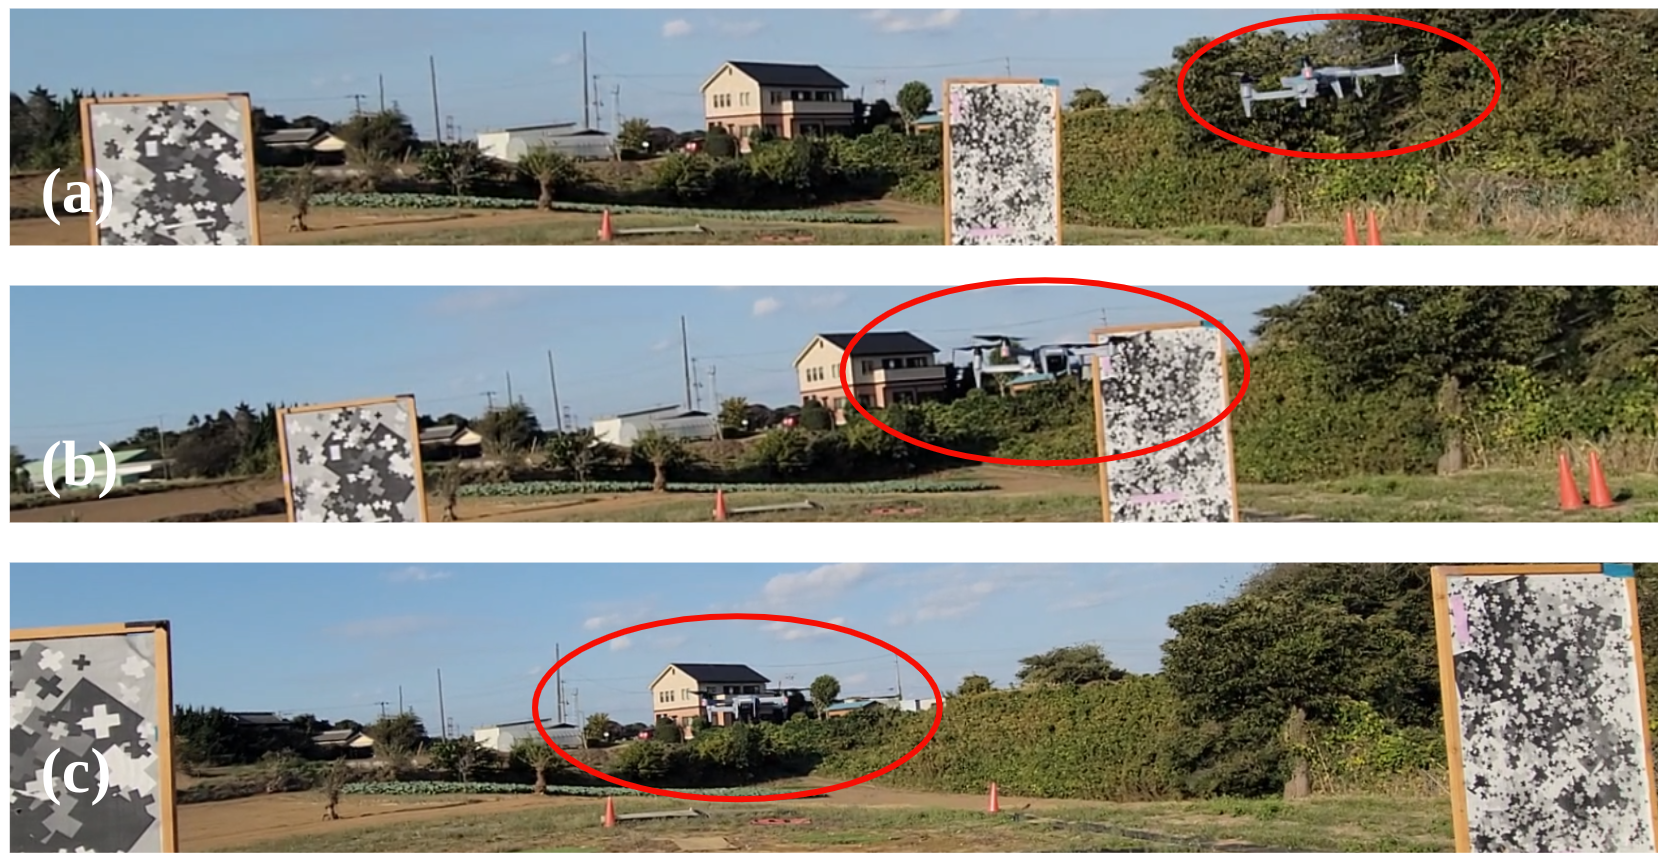
\includegraphics[scale=0.25]{partes/img/real-3-parallelB-1-frames.png}
    \caption[Capturas de la grabación del vuelo en entorno real con obstáculos paralelos a 4 metros de separación.]{Capturas de la grabación del vuelo en entorno real con obstáculos paralelos a 4 metros de separación. \textbf{(a)} La ejecución comienza y el QUAV navega hacia el espacio entre los dos obstáculos. \textbf{(b)} El obstáculo izquierdo sale del campo de visión, y el QUAV continúa hacia el espacio entre los dos obstáculos. \textbf{(c)}  Se superan los obstáculos y se navega en dirección a la meta.}
    \label{real-3-parallelB-1-frames}
\end{figure}

\begin{figure}[H]
    \centering
    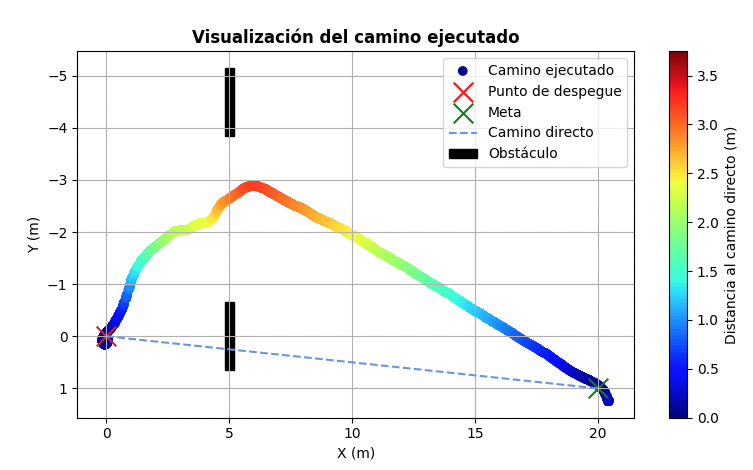
\includegraphics[scale=0.5]{partes/img/real-3-parallelB-2-graph.png}
    \caption[Visualización del camino ejecutado por el QUAV para la configuración de obstáculos paralelos a 4 metros de separación en entorno real.]{Visualización del camino ejecutado por el QUAV para la configuración de obstáculos paralelos a 4 metros de separación en entorno real.}
    \label{real-3-parallelB-2-graph}
\end{figure}

El tercer y último vuelo en la configuración de obstáculos paralelos utilizó una separación de un metro, la Figura \ref{real-4-parallelC-0-config} muestra una fotografía que ilustra la configuración utilizada. Este vuelo resultó exitoso y la razón por la cual fue exitoso provee información adicional sobre la capacidad de evasión de obstáculos del algoritmo. La Figura \ref{real-4-parallelC-1-frames} muestra capturas de la grabación de este vuelo en donde se observa el comportamiento del algoritmo. Primero (Figura \ref{real-4-parallelC-1-frames}(a)), la ejecución comienza y el QUAV navega hacia el espacio entre los dos obstáculos; segundo (Figura \ref{real-4-parallelC-1-frames}(b)), en el momento que el obstáculo izquierdo se vuelve el obstáculo mas grande en el campo de visión, el algoritmo intenta fuertemente corregir la trayectoria para esquivar el conjunto de obstáculos por el flanco izquierdo del obstáculo izquierdo, esto ocurre tempranamente en el vuelo pues la separación entre los obstáculos es relativamente pequeña; y tercero (Figura \ref{real-4-parallelC-1-frames}(c)), como la decisión de de corregir la trayectoria hacia la izquierda ocurre de forma temprana, el algoritmo tiene tiempo de completar la trayectoria sin producir colisiones, resultando en una ejecución exitosa. La Figura \ref{real-4-parallelC-2-graph} muestra una visualización de arriba hacia abajo del camino ejecutado por el QUAV en esta configuración, en donde se evidencia el momento en el que el algoritmo intenta corregir fuertemente; adicionalmente, para respladar la magnitud de la corrección en la Figura \ref{real-4-parallelC-3-yaw} se muestra el grafico del encabezamiento del QUAV en función del tiempo, en donde se observan oscilaciones de relativamente alta magnitud. El resultado de este vuelo expone que si existe el espacio y el tiempo para esquivar un conjunto de obstáculos por el flanco mas hacia la izquierda, es posible que la política de evasión de obstáculos sea capaz de completar el vuelo exitosamente.

\begin{figure}[H]
    \centering
    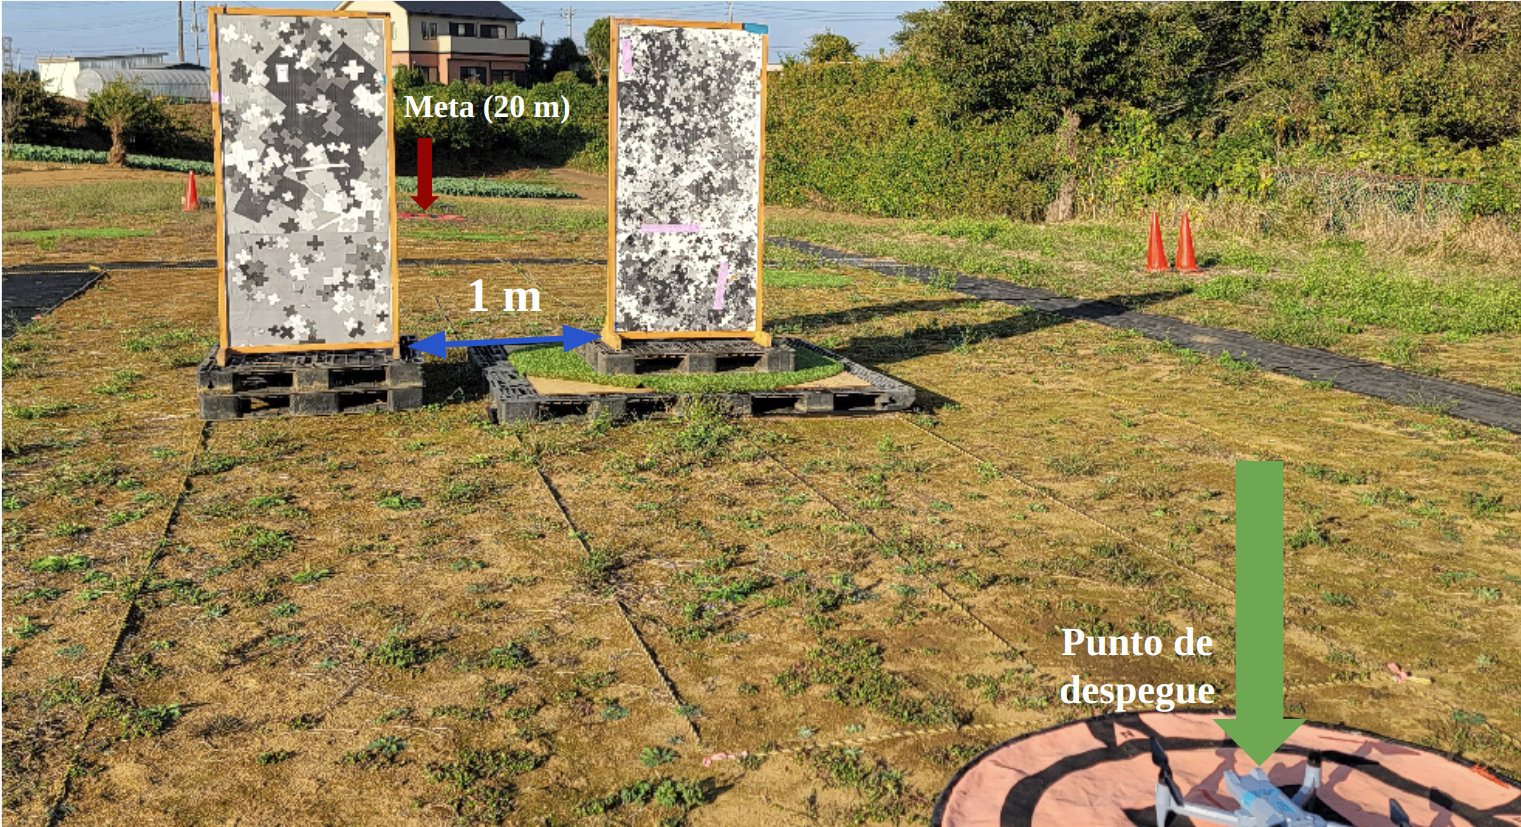
\includegraphics[scale=0.25]{partes/img/real-4-parallelC-0-config.png}
    \caption[Configuración de obstáculos en entorno real: Obstáculos paralelos a 1 metro de separación.]{Configuración de obstáculos en entorno real: Obstáculos paralelos a 1 metro de separación.}
    \label{real-4-parallelC-0-config}
\end{figure}

\begin{figure}[H]
    \centering
    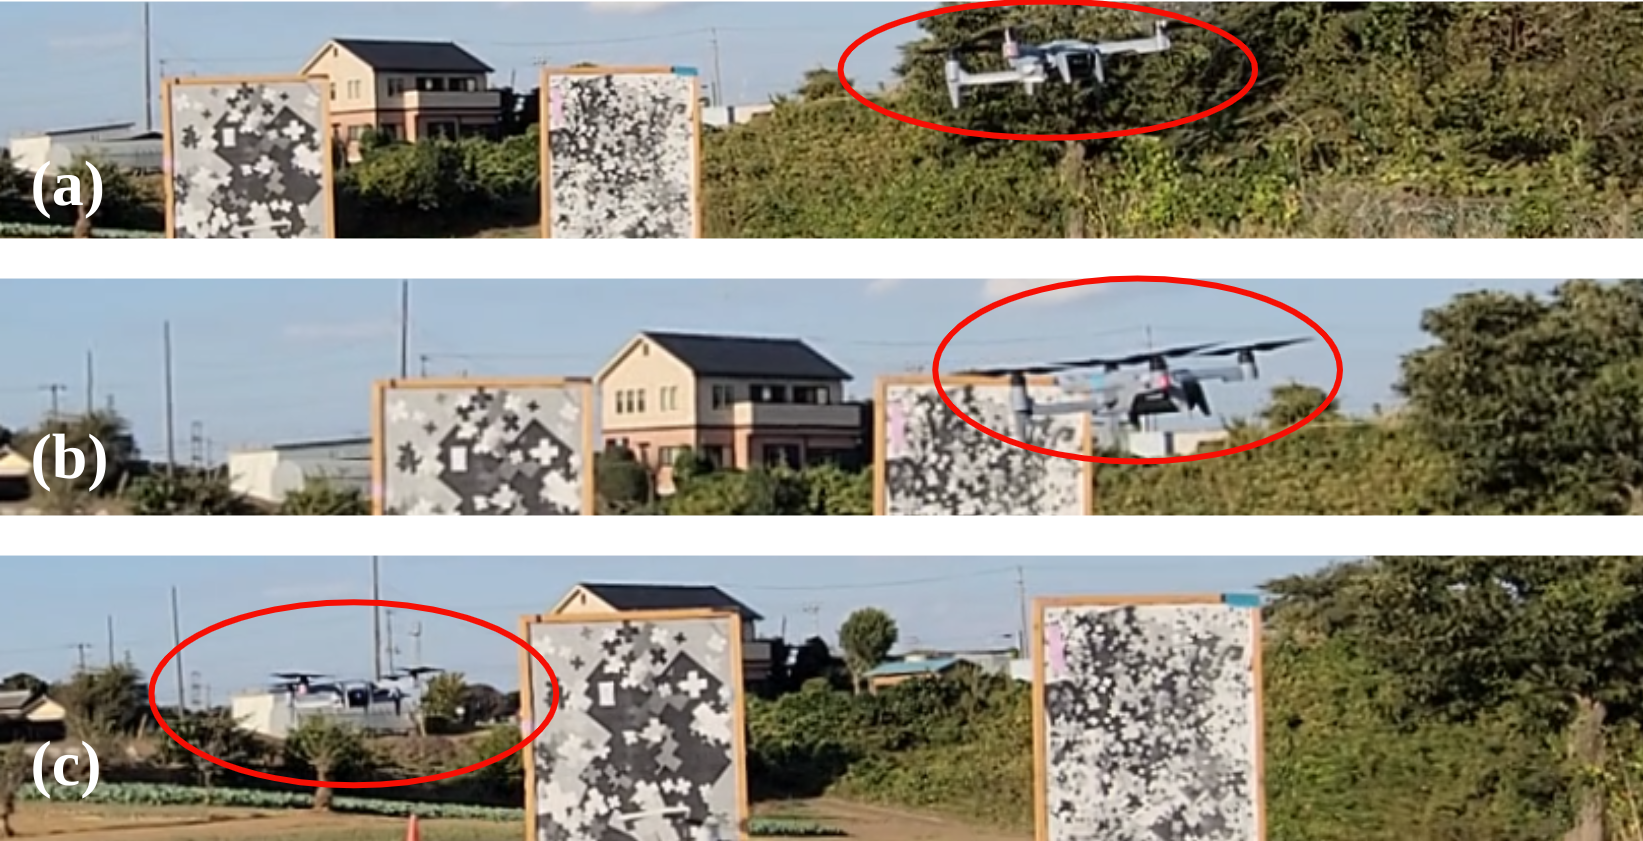
\includegraphics[scale=0.24]{partes/img/real-4-parallelC-1-frames.png}
    \caption[Capturas de la grabación del vuelo en entorno real con obstáculos paralelos a 1 metro de separación.]{Capturas de la grabación del vuelo en entorno real con obstáculos paralelos a 1 metro de separación. \textbf{(a)} La ejecución comienza y el QUAV navega hacia el espacio entre los dos obstáculos. \textbf{(b)} El obstáculo izquierdo se vuelve el obstáculo mas grande en el campo de visión y el algoritmo intenta fuertemente corregir la trayectoria para esquivar el conjunto de obstáculos por el flanco izquierdo del obstáculo izquierdo. \textbf{(c)} Como la decisión de de corregir la trayectoria hacia la izquierda ocurre de forma temprana, el algoritmo tiene tiempo de completar la trayectoria sin producir colisiones, resultando en una ejecución exitosa. }
    \label{real-4-parallelC-1-frames}
\end{figure}

\begin{figure}[H]
    \centering
    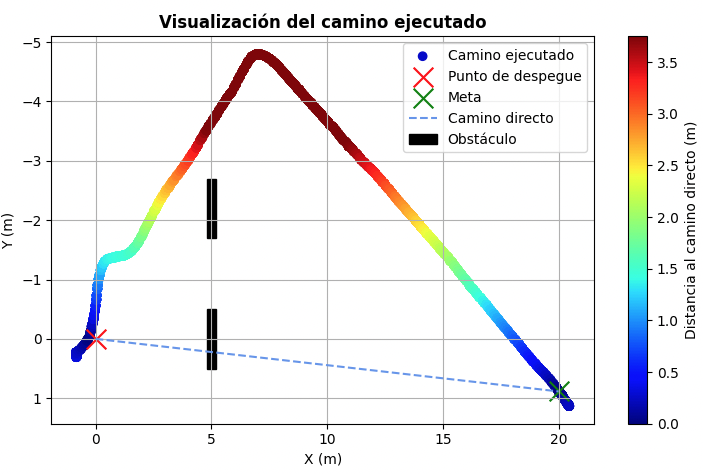
\includegraphics[scale=0.5]{partes/img/real-4-parallelC-2-graph.png}
    \caption[Visualización del camino ejecutado por el QUAV para la configuración de obstáculos paralelos a 1 metro de separación en entorno real.]{Visualización del camino ejecutado por el QUAV para la configuración de obstáculos paralelos a 1 metro de separación en entorno real. Se puede observar el momento en el que el algoritmo intenta corregir fuertemente la trayectoria hacia la izquierda.}
    \label{real-4-parallelC-2-graph}
\end{figure}

\begin{figure}[H]
    \centering
    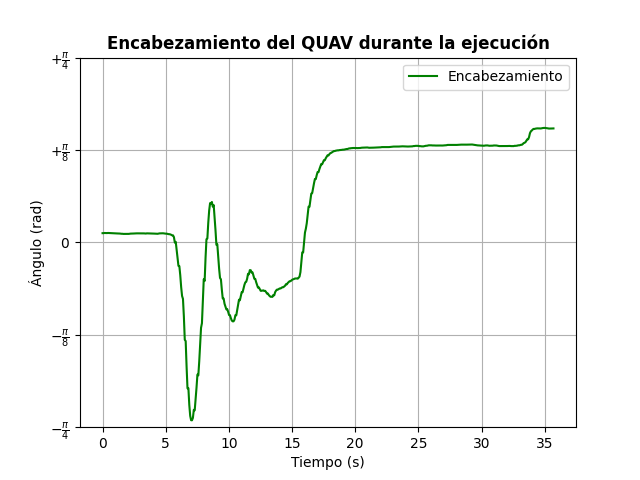
\includegraphics[scale=0.8]{partes/img/real-4-parallelC-3-yaw.png}
    \caption[Grafico del encabezamiento del QUAV en función del tiempo para la configuración de obstáculos paralelos a 1 metro de separación en entorno real.]{Grafico del encabezamiento del QUAV en función del tiempo para la configuración de obstáculos paralelos a 1 metro de separación en entorno real. Se observan oscilaciones de relativamente alta magnitud que corresponden al momento en el que el algoritmo intenta corregir fuertemente la trayectoria hacia la izquierda.}
    \label{real-4-parallelC-3-yaw}
\end{figure}

Los vuelos realizados permiten evaluar la estabilidad del algoritmo de evasión de obstáculos en entornos de la vida real, resaltando su consistencia, especialmente en la configuración de un obstáculo simple. No obstante, los resultados también revelan los efectos derivados de las dificultades encontradas durante el refinamiento fino de la política estudiante, manifestándose principalmente en la preferencia absoluta por esquivar obstáculos hacia el flanco izquierdo. Como consecuencia directa de estos vuelos, se exploran escenarios que ilustran el impacto de esta preferencia en situaciones de la vida real que involucran configuraciones de dos obstáculos paralelos. Dicho esto, finalmente, en la Tabla \ref{table:real-results} se muestra un resumen de los resultados obtenidos en los vuelos en entornos de la vida real.

\begin{table}[h]
\centering
\begin{tabular}{||c || c | c | c | c | c | c||} 
 \hline
 \textbf{Configuración} & \jim{N} & \jim{N_{e}} & \textbf{P} & \jim{\bar{D}} & \jim{\max(D)} & \jim{\min(D)} \rule{0pt}{2.6ex} \\ [0.4ex] 
 \hline\hline
 Obstáculo simple              & 11 & 10 & \textbf{90\%} & 3.2 & 4.5 & 2 \\ 
 \hline
 Dos obstáculos paralelos      & 3 &  2  & \textbf{66\%} & 4 & 4.9 & 3.1 \\
 \hline
\end{tabular}
\caption[Resumen de los resultados obtenidos en los vuelos en entornos de la vida real.]{Resumen de los resultados obtenidos en los vuelos en entornos de la vida real. \jim{N} y \jim{N_{e}} son el número de vuelos totales y sin colisión inminente respectivamente. \textbf{P} es el porcentaje de vuelos sin colisión inminente. \jim{\bar{D}}, \jim{\max(D)} y \jim{\min(D)} son la desviación máxima promedio, máxima y mínima respectivamente (en metros).}
\label{table:real-results}
\end{table}

\section{Resumen}

Este capítulo abordó la evaluación y presentación de los resultados obtenidos, proporcionando una perspectiva crítica sobre el rendimiento de la solución propuesta. En la Sección \ref{sec:results-finetune}, se exploraron los resultados del ajuste fino de la política estudiante, destacando los desafíos asociados al sobre-ajuste de los datos de entrenamiento y a la generación de la base de datos. Además, se aclaró que, debido a limitaciones de tiempo de desarrollo y recomendaciones del equipo de ACSL, no se abordó completamente el problema del sobre-ajuste, lo que produjo efectos evidentes al evaluar la política de evasión de obstáculos. En particular, se observó cómo esta decisión ha llevado a una fuerte preferencia de la política por esquivar obstáculos por el flanco izquierdo.

La Sección  \ref{sec:results-flights} detalló los resultados de la política de evasión de obstáculos, presentando los vuelos en simulación en la Sección  \ref{sec:results-AirSim} y los vuelos sobre la plataforma física de implementación, SOTEN, en la Sección  \ref{sec:results-SOTEN}. Estos resultados ofrecieron una perspectiva del rendimiento de la solución en configuraciones simples de obstáculos, donde la política de evasión se mostró estable. También se exploraron configuraciones donde la fuerte preferencia de la política por esquivar obstáculos por el flanco izquierdo produjo colisiones, y se observaron distintos escenarios y consecuencias de ello.

En resumen, este capítulo proporcionó una evaluación que sirve de base para la discusión del siguiente capítulo, el de conclusiones. El contexto introducido en este capítulo también permite considerar direcciones para trabajos futuros que se construyan sobre la implementación presentada en este trabajo.
